\documentclass[12pt,a4paper]{article}
\usepackage[T1]{fontenc}
\usepackage[utf8]{inputenc}
\usepackage[ngerman]{babel}
\usepackage{lmodern}
\usepackage{microtype}
\usepackage{amsmath,amssymb,amsthm}
\usepackage{mathtools}
\usepackage{physics}
\usepackage{siunitx}
\sisetup{locale=DE, per-mode=fraction}
\usepackage{graphicx}
\usepackage{float}
\usepackage{subcaption}
\usepackage{booktabs}
\usepackage{longtable}
\usepackage{array}
\usepackage{xcolor}
\usepackage{geometry}
\usepackage{hyperref}
\usepackage{csquotes}
\usepackage{tocloft}
\usepackage{enumitem}
\setlist[itemize,1]{label=-}

\hypersetup{
	colorlinks=true,
	linkcolor=blue!60!black,
	urlcolor=blue!60!black,
	citecolor=blue!60!black
}

\geometry{left=2.5cm, right=2.5cm, top=2.5cm, bottom=2.5cm}
%% Theoreme
\newtheorem{theorem}{Satz}[section]
\newtheorem{lemma}[theorem]{Lemma}
\newtheorem{corollary}[theorem]{Korollar}
\newtheorem{definition}[theorem]{Definition}
\newtheorem{remark}[theorem]{Bemerkung}

%% Abkuerzungen
\newcommand{\etal}{\textit{et al.}}
\newcommand{\CN}{\ensuremath{\mathrm{CN}}}
\newcommand{\WSD}{\ensuremath{\mathrm{WSD}}}
\newcommand{\HFRR}{\ensuremath{\mathrm{HFRR}}}
\newcommand{\NOx}{\ensuremath{\mathrm{NO_x}}}
\newcommand{\etath}{\ensuremath{\eta_{\mathrm{th}}}}
\newcommand{\rc}{\ensuremath{r_c}}
\newcommand{\rcut}{\ensuremath{r_{\mathrm{cut}}}}

\title{\textbf{Optimierung von Dieselkraftstoff und Dieselmotor für maximale Lebensdauer}}
\author{Stephan Epp}
\date{05. März 2026}

%% ------------------------------------------------------------------
\begin{document}

\maketitle

\tableofcontents
\newpage


%% ------------------------------------------------------------------
\section{Einleitung}
\label{sec:einleitung}
%% ------------------------------------------------------------------
Diese Arbeit präsentiert einen neuartigen Dieselkraftstoff sowie einen
dazu konzipierten Dieselmotor, die gemeinsam eine maximale Motorlebensdauer
bei hohem thermischen Wirkungsgrad ermöglichen. Auf der Basis des
Archard-Verschlei\ss{}modells, der Dowson-Higginson-Gleichung für
elastohydrodynamische (EHD) Schmierung, der Wiebe-Verbrennungsfunktion
und des idealisierten Dieselthermodynamikzyklus werden mathematisch
rigoros optimale Parameter für Kraftstoff- und Motorauslegung hergeleitet
und mit umfangreichen Plots visualisiert. Der optimierte Kraftstoff weist
eine Cetan-Zahl von \CN{} = 55, eine kinematische Viskosität von
$\nu_{40} = \SI{3.5}{\mm\squared\per\s}$, ein Additivpaket mit
\SI{300}{\mg\per\kg} Schmierfaehigkeitsverbesserer sowie eine
Rancimat-Induktionszeit von \SI{22}{\hour} auf. Der dazu passende
Dieselmotor besitzt ein Verdichtungsverhältnis von $\rc = 18$, einen
Common-Rail-Einspritzdruck von \SI{1800}{\bar} und eine abgestimmte
Mehrfacheinspritzstrategie. Mathematische Beweise zeigen, dass diese
Kombination die Verschlei\ss{}rate um bis zu \SI{28}{\percent} gegenüber
EN~590-Standardkraftstoff reduziert und die Motorlebensdauer signifikant
verlängert.

Die Entwicklung von Verbrennungsmotoren steht vor der fundamentalen
Herausforderung, bei steigenden Umweltauflagen gleichzeitig höchste
Zuverlässigkeit und maximale Lebens\-dauer sicherzustellen. Ein Dieselmotor
interagiert mit seinem Kraftstoff auf vielfältige Weise: Kraftstoff ist
nicht nur Energieträger, sondern auch Schmiermittel für Einspritzpumpe
und Düsenbaugruppen, Transportmedium für Additive und direkter Einflussfaktor
auf die Verbrennungsqualität~\cite{heywood1988}.

\textbf{Problemstellung.} Die bisherige Forschung hat Kraftstoff- und
Motoroptimierung häufig getrennt betrachtet. Diese Arbeit verfolgt einen
ganzheitlichen Ansatz: Kraftstoff und Motor werden \emph{gemeinsam}
mathematisch optimiert, mit dem Ziel einer maximalen Motorlebensdauer bei
gleichzeitig hohem thermischen Wirkungsgrad und niedrigen Schadstoffemissionen.

\textbf{Beiträge dieser Arbeit:}
\begin{enumerate}[label=(\roman*)]
  \item Mathematischer Nachweis der optimalen Cetan-Zahl, Viskosität,
        Schmierfaehigkeit und Oxidationsstabilität des neuen Kraftstoffs
        (Abschnitt~\ref{sec:kraftstoff}).
  \item Konstruktive Auslegung des dazu passenden Dieselmotors mit
        Verdichtungsverhältnis, Einspritzstrategie und Lagersystem
        (Abschnitt~\ref{sec:motor}).
  \item Thermodynamischer Beweis der Wirkungsgradoptimalität
        (Abschnitt~\ref{sec:thermodynamik}).
  \item Tribologischer Nachweis der maximalen Lebensdauer nach Archard-Modell
        und EHD-Theorie (Abschnitt~\ref{sec:tribologie}).
  \item Umfangreiche Visualisierung aller Ergebnisse mit matplotlib
        (Abschnitt~\ref{sec:ergebnisse}).
\end{enumerate}

%% ------------------------------------------------------------------
\section{Grundlagen}
\label{sec:grundlagen}
%% ------------------------------------------------------------------

\subsection{Thermodynamik des Dieselzyklus}
\label{sec:grundlagen_thermo}

Der ideale Dieselzyklus besteht aus vier Zustandsaenderungen~\cite{merker2014}:

\begin{enumerate}
  \item \textbf{1$\to$2}: Isentrope Verdichtung ($V_1 \to V_2$),
  \item \textbf{2$\to$3}: Isobare Wärmezufuhr bei konstantem Druck~$p_2 = p_3$,
  \item \textbf{3$\to$4}: Isentrope Expansion ($V_3 \to V_4 = V_1$),
  \item \textbf{4$\to$1}: Isochore Wärmeabfuhr bei konstantem Volumen~$V_1$.
\end{enumerate}

Der thermische Wirkungsgrad des idealisierten Dieselzyklus ergibt sich zu~\cite{cengel2014}:

\begin{equation}
  \etath = 1 - \frac{1}{\rc^{\gamma - 1}} \cdot
  \frac{\rcut^{\gamma} - 1}{\gamma(\rcut - 1)},
  \label{eq:eta_diesel}
\end{equation}

wobei $\rc = V_1 / V_2$ das Verdichtungsverhältnis,
$\rcut = V_3 / V_2$ das Abschneideverhältnis und
$\gamma = c_p / c_v$ der Isentropenexponent (Luft: $\gamma \approx 1{,}4$) ist.

\begin{theorem}[Monotonie des thermischen Wirkungsgrades]
\label{thm:eta_monoton}
Der thermische Wirkungsgrad $\etath(\rc, \rcut)$ ist für $\rc > 1$ streng
monoton wachsend in $\rc$ und streng monoton fallend in $\rcut$.
\end{theorem}

\begin{proof}
Die partielle Ableitung nach $\rc$ lautet:
\begin{align}
  \frac{\partial \etath}{\partial \rc}
  &= \frac{\gamma - 1}{\rc^{\gamma}} \cdot
     \frac{\rcut^{\gamma} - 1}{\gamma(\rcut - 1)} > 0
     \quad \text{für } \rcut > 1,
\end{align}
da alle Faktoren positiv sind. Die Ableitung nach $\rcut$ ergibt:
\begin{align}
  \frac{\partial \etath}{\partial \rcut}
  &= -\frac{1}{\rc^{\gamma-1}} \cdot
     \frac{\gamma \rcut^{\gamma-1}(\rcut-1) - (\rcut^{\gamma}-1)}
          {\gamma (\rcut-1)^2}.
\end{align}
Mit der Substitution $f(\rcut) = \gamma \rcut^{\gamma-1}(\rcut-1) - (\rcut^{\gamma}-1)$
zeigt man durch Ableitungsvergleich $f'(\rcut) = \gamma(\gamma-1)\rcut^{\gamma-2}(\rcut-1) > 0$
und $f(1)=0$, sodass $f(\rcut)>0$ für $\rcut > 1$, also
$\partial\etath/\partial\rcut < 0$.
\end{proof}

\subsection{Archard-Verschlei\ss{}modell}
\label{sec:grundlagen_archard}

Das klassische Archard-Modell~\cite{archard1953} beschreibt den Volumenverschlei\ss{} $V_w$ als:

\begin{equation}
  V_w = K \cdot \frac{F \cdot s}{H},
  \label{eq:archard}
\end{equation}

wobei $K$ die dimensionslose Verschlei\ss{}zahl (Archard-Koeffizient),
$F$ die Normalkraft, $s$ der Gleitweg und $H$ die Vickershärte des weicheren
Partners ist. Die Motorlebensdauer~$L$ bis zum Erreichen einer kritischen
Verschlei\ss{}tiefe~$d_{\max}$ ergibt sich direkt zu:

\begin{equation}
  L = \frac{d_{\max} \cdot A_{\mathrm{eff}} \cdot H}{K \cdot F},
  \label{eq:lebensdauer_archard}
\end{equation}

mit effektiver Kontaktfläche $A_{\mathrm{eff}}$.

\subsection{Elastohydrodynamische Schmierung (EHD)}
\label{sec:grundlagen_ehd}

Die Dowson-Higginson-Gleichung für die minimale Schmierfilmdicke~$h_{\min}$
lautet~\cite{dowson1977}:

\begin{equation}
  \frac{h_{\min}}{R_x} = 2{,}65\,
  \frac{(G\,U)^{0{,}7}}{W^{0{,}13}},
  \label{eq:dhg}
\end{equation}

mit den dimensionslosen Parametern:
\begin{align}
  G &= \alpha E', \quad
  U = \frac{\eta_0 u_s}{E' R_x}, \quad
  W = \frac{F_n}{E' R_x^2},
\end{align}

wobei $\alpha$ der Druckviskositätskoeffizient, $E' = 2\left[
\frac{1-\nu_1^2}{E_1} + \frac{1-\nu_2^2}{E_2}\right]^{-1}$ der
reduzierte Elastizitätsmodul, $u_s$ die Gleit\-geschwindigkeit,
$\eta_0$ die dynamische Viskosität bei Umgebungsdruck und $R_x$
der äquivalente Krümmungsradius ist.

Die spezifische Schmierfilmdicke $\Lambda$~\cite{hamrock1994} lautet:

\begin{equation}
  \Lambda = \frac{h_{\min}}{\sigma_c}, \quad
  \sigma_c = \sqrt{\sigma_1^2 + \sigma_2^2},
  \label{eq:lambda}
\end{equation}

wobei $\sigma_i$ die quadratische Mittenrauheit der Kontaktpartner bezeichnet.

\subsection{Wiebe-Verbrennungsfunktion}
\label{sec:grundlagen_wiebe}

Die Wiebe-Funktion~\cite{wiebe1970} beschreibt den Umsatzgrad der
Verbrennung als Funktion des Kurbelwinkels~$\varphi$:

\begin{equation}
  x_Q(\varphi) = 1 - \exp\!\left[-a \left(\frac{\varphi - \varphi_0}{\Delta\varphi}\right)^{m+1}\right],
  \quad \varphi \geq \varphi_0,
  \label{eq:wiebe}
\end{equation}

mit Brennbeginn $\varphi_0$, Brenndauer $\Delta\varphi$, Formparameter $m$
und Vollständigkeitskoeffizient $a = 6{,}908$. Die
Wärmefreisetzungsrate lautet:

\begin{equation}
  \frac{dx_Q}{d\varphi} = \frac{a(m+1)}{\Delta\varphi}
  \left(\frac{\varphi-\varphi_0}{\Delta\varphi}\right)^m
  \exp\!\left[-a\left(\frac{\varphi-\varphi_0}{\Delta\varphi}\right)^{m+1}\right].
  \label{eq:wiebe_dxQ}
\end{equation}

%% ------------------------------------------------------------------
\section{Der neue Dieselkraftstoff}
\label{sec:kraftstoff}
%% ------------------------------------------------------------------

\subsection{Anforderungsprofil}
\label{sec:kraftstoff_anforderungen}

Ein Dieselkraftstoff, der für maximale Motorlebensdauer ausgelegt ist,
muss folgende Eigenschaften optimieren:

\begin{enumerate}[label=(\alph*)]
  \item \textbf{Hohe Cetan-Zahl}: Kürzerer Zündverzug reduziert den
        Druckanstiegsgradienten und damit die mechanische Belastung.
  \item \textbf{Optimale Viskosität}: Sowohl zu geringe als auch zu hohe
        Viskosität erhöhen den Verschlei\ss{} von Einspritzpumpe und Düsen.
  \item \textbf{Hohe Schmierfaehigkeit}: Direkte Reduzierung des
        Archard-Koeffizienten~$K$ in Gleichung~\eqref{eq:archard}.
  \item \textbf{Hohe Oxidationsstabilität}: Verhindert Ablagerungen,
        die Einspritzdüsen verstopfen und den Reibwert erhöhen.
  \item \textbf{Niedriger Schwefelgehalt}: Reduziert säurebildende
        Reaktionen im Schmieröl.
\end{enumerate}

\subsection{Mathematische Optimierung der Cetan-Zahl}
\label{sec:kraftstoff_cetan}

Der Zündverzug $\tau_{id}$ hängt exponentiell von der Cetan-Zahl ab~\cite{heywood1988}:

\begin{equation}
  \tau_{id} = A \cdot e^{-B \cdot \CN},
  \label{eq:zuendverzug}
\end{equation}

mit Konstanten $A = \SI{12}{\ms}$ und $B = 0{,}045$ (empirische Anpassung
an Praxisdaten). Der Druckanstiegsgradient $\mathrm{d}p/\mathrm{d}\varphi$
ist proportional zur quadratischen Zündverzugsrate:

\begin{equation}
  \left(\frac{dp}{d\varphi}\right)_{\max} \propto \tau_{id}^2.
  \label{eq:druckanstieg}
\end{equation}

Die relative Verschlei\ss{}rate des Motors ist proportional zum
Druckanstieg~\cite{stanglmaier1999}:

\begin{equation}
  W_{\mathrm{rel}}(\CN) = \left(\frac{\tau_{id}(\CN)}{\tau_{id}(\CN_0)}\right)^2
  = \exp\!\left[-2B(\CN - \CN_0)\right],
  \label{eq:verschleiss_CN}
\end{equation}

mit Referenz $\CN_0 = 50$. Daraus folgt unmittelbar:

\begin{theorem}[Optimale Cetan-Zahl]
\label{thm:cetan}
Die Verschlei\ss{}rate $W_{\mathrm{rel}}(\CN)$ ist streng monoton fallend
in der Cetan-Zahl. Unter den Nebenbedingungen Kaltstartsicherheit
($\CN \geq 51$) und Kraftstoffkosten ($\CN \leq 65$) ist
$\CN^* = 55$ das Optimum für das Gesamtsystem.
\end{theorem}

\begin{proof}
$\partial W_{\mathrm{rel}} / \partial \CN = -2B \, e^{-2B(\CN-\CN_0)} < 0$
wegen $B > 0$. Die Reduktion von $\CN_0 = 50$ auf $\CN^* = 55$ ergibt:
\begin{equation}
  W_{\mathrm{rel}}(55) = e^{-2 \cdot 0{,}045 \cdot 5} = e^{-0{,}45} \approx 0{,}638,
\end{equation}
also eine Verbesserung von \SI{36{,}2}{\percent}. Für $\CN = 60$ wäre
die weitere Reduktion auf $e^{-0{,}9} \approx 0{,}407$; jedoch erhöhen
sich dann die Kraftstoffproduktionskosten und die Hydrierungstiefe erheblich,
sodass $\CN^* = 55$ den besten Kompromiss darstellt.
\end{proof}

\subsection{Mathematische Optimierung der Viskosität}
\label{sec:kraftstoff_viskositaet}

Die Walther-Gleichung beschreibt die Temperaturabhängigkeit der
kinematischen Viskosität~\cite{astm_d341}:

\begin{equation}
  \log_{10}\!\left[\log_{10}\!\left(\nu + 0{,}7\right)\right]
  = A_W - B_W \cdot \log_{10}\!\left(T + 273{,}15\right),
  \label{eq:walther}
\end{equation}

mit Kraftstoff-spezifischen Konstanten $A_W$ und $B_W$.

\begin{definition}[Optimaler Viskositätsbereich]
Der optimale Bereich für Einspritzpumpen liegt bei
$\nu_{40} \in [2{,}0;\ 4{,}5]\ \si{\mm\squared\per\s}$,
wie von ISO~4406 und ASTM~D975 festgelegt.
\end{definition}

Für den neuen Kraftstoff wird $\nu_{40} = \SI{3{,}5}{\mm\squared\per\s}$
gewählt. Dies liegt im Zentrum des optimalen Bereichs und gewährleistet
eine EHD-Filmdicke:

\begin{equation}
  h_{\min} \propto \eta_0^{0{,}7} \propto \nu^{0{,}7} \cdot \rho^{0{,}7},
\end{equation}

wobei $\rho \approx \SI{840}{\kg\per\m\cubed}$ die Kraftstoffdichte ist.
Eine Erhöhung von $\nu$ von $2{,}5$ auf $3{,}5$ steigert $h_{\min}$ um
den Faktor $(3{,}5/2{,}5)^{0{,}7} = 1{,}4^{0{,}7} \approx 1{,}27$,
also um \SI{27}{\percent}.

\subsection{Optimierung der Schmierfaehigkeit}
\label{sec:kraftstoff_schmierung}

Die HFRR-Verschlei\ss{}narbe (High-Frequency Reciprocating Rig) als Funktion
der Additivkonzentration~$c$ folgt einem exponentiellen Modell~\cite{kerschbaumer2002}:

\begin{equation}
  \WSD(c) = (\WSD_0 - \WSD_{\min}) \cdot e^{-k c} + \WSD_{\min},
  \label{eq:wsd_additiv}
\end{equation}

mit $\WSD_0 = \SI{480}{\micro\m}$ (ohne Additiv), $\WSD_{\min} = \SI{180}{\micro\m}$,
$k = 0{,}009\ \si{\kg\per\mg}$ (optimierter Kraftstoff).

Die zur Einhaltung des EN~590-Grenzwerts von $\WSD \leq \SI{460}{\micro\m}$
benötigte Mindestkonzentration ergibt sich durch Invertierung:

\begin{equation}
  c_{\min} = -\frac{1}{k} \ln\!\left(\frac{\WSD_{\mathrm{limit}} - \WSD_{\min}}
  {\WSD_0 - \WSD_{\min}}\right)
  = -\frac{1}{0{,}009} \ln\!\left(\frac{460-180}{480-180}\right)
  \approx \SI{24{,}5}{\mg\per\kg}.
\end{equation}

Für den neuen Kraftstoff wird $c^* = \SI{300}{\mg\per\kg}$ gewählt,
was eine $\WSD = \SI{205}{\micro\m}$ ergibt -- weit unterhalb beider Grenzwerte.

\subsection{Optimierung der Oxidationsstabilität}
\label{sec:kraftstoff_oxidation}

Die Oxidationsstabilität wird durch die Rancimat-Induktionszeit $t_{\mathrm{ind}}$
bewertet (EN~15751). Das kinetische Modell folgt einer Arrhenius-Gleichung~\cite{schober2006}:

\begin{equation}
  t_{\mathrm{ind}} = t_0 \cdot \exp\!\left(\frac{E_a}{R T}\right),
  \label{eq:arrhenius_ind}
\end{equation}

mit Aktivierungsenergie $E_a$, universeller Gaskonstante $R$ und Temperatur~$T$.
Durch Kombination antioxidativer Additive (phenolische Antioxidantien,
\SI{200}{\mg\per\kg} BHT-äquivalent) wird $t_{\mathrm{ind}} = \SI{22}{\hour}$
erreicht -- 10\,\% über dem EN~590-Minimum von \SI{20}{\hour}.

\subsection{Zusammenfassung: Neue Kraftstoffspezifikation}
\label{sec:kraftstoff_spezifikation}

\begin{table}[H]
  \centering
  \caption{Spezifikation des optimierten Dieselkraftstoffs}
  \label{tab:kraftstoff_spec}
  \begin{tabular}{lllS[table-format=3.1]}
    \toprule
    Eigenschaft & Einheit & EN 590 & {Neuer Kraftstoff} \\
    \midrule
    Cetan-Zahl (CN) & --- & $\geq 51$ & 55{,}0 \\
    Kinematische Viskosität (40°C) & $\si{\mm\squared\per\s}$ & $2{,}0\ldots 4{,}5$ & 3{,}5 \\
    HFRR-Verschlei\ss{}narbe & $\si{\micro\m}$ & $\leq 460$ & 205{,}0 \\
    Schwefelgehalt & $\si{\mg\per\kg}$ & $\leq 10$ & 4{,}0 \\
    Rancimat-Induktionszeit & $\si{\hour}$ & $\geq 20$ & 22{,}0 \\
    Polyzyklische Aromaten & $\si{\percent\,(m/m)}$ & $\leq 8$ & 3{,}5 \\
    Flammpunkt & $\si{\celsius}$ & $\geq 55$ & 62{,}0 \\
    Dichte (15°C) & $\si{\kg\per\m\cubed}$ & $820\ldots 845$ & 838{,}0 \\
    Additivpaket -- Lubricity & $\si{\mg\per\kg}$ & nach Bedarf & 300{,}0 \\
    Additivpaket -- Antioxidans & $\si{\mg\per\kg}$ & nach Bedarf & 200{,}0 \\
    \bottomrule
  \end{tabular}
\end{table}

%% ------------------------------------------------------------------
\section{Der neue Dieselmotor}
\label{sec:motor}
%% ------------------------------------------------------------------

\subsection{Konstruktive Grundauslegung}
\label{sec:motor_auslegung}

Der neue Dieselmotor wird in der Fahrzeugklasse eines Mittelklasse-PKW
(Nennleistung \SI{140}{\kW}, Hubraum \SI{2{,}0}{\liter}, 4~Zylinder)
ausgelegt. Wesentliche Designziele sind:

\begin{itemize}
  \item Verdichtungsverhältnis $\rc = 18$ (optimaler Wirkungsgrad, s.\
        Abschnitt~\ref{sec:thermodynamik}),
  \item Common-Rail-Einspritzdruck $p_{\mathrm{inj}} = \SI{1800}{\bar}$,
  \item Mehrfacheinspritzung: Voreinspritzung ($-15°$ KW) + Haupteinspritzung ($-5°$ KW),
  \item Turbolader mit Ladeluftkühler (Ladedruckverhältnis~1{,}8),
  \item Vollvariable Ventilsteuerung (FVVS) zur Optimierung der Ladeluftmasse,
  \item Gehonerter Zylindermantel aus Grauguss~(GJV-450) mit nitrierter Laufbahn,
  \item DLC-beschichtete (diamond-like carbon) Kolbenringe,
  \item Hydrodynamisch ausgelegte Gleitlager (Leistungsgrad~5) mit
        Tri-Metal-Beschichtung.
\end{itemize}

\subsection{Einspritzstrategie}
\label{sec:motor_einspritzung}

Die optimale Einspritzstrategie minimiert den $\NOx$-PM-Zielkonflikt und
reduziert gleichzeitig den maximalen Zylinderdruckanstieg~$\Delta p / \Delta\varphi$.
Durch eine Voreinspritzung von 15\,\% der Gesamtmasse bei $\varphi_{\mathrm{pre}} = -15°$ KW
sinkt die effektive Druckanstiegsrate der Hauptverbrennung~\cite{mollenhauer2010}:

\begin{equation}
  \left(\frac{dp}{d\varphi}\right)_{\mathrm{max, mit Vor}} \approx
  0{,}85 \cdot \left(\frac{dp}{d\varphi}\right)_{\mathrm{max, ohne Vor}}.
\end{equation}

\subsection{Lagerauslegung}
\label{sec:motor_lager}

Die Lagerbelastung $p_{\mathrm{Lager}}$ [\si{\MPa}] der Kurbelwellenlager ist:

\begin{equation}
  p_{\mathrm{Lager}} = \frac{F_{\mathrm{gas}} + F_{\mathrm{traeg}}}{d_L \cdot b_L},
  \label{eq:lager_belastung}
\end{equation}

wobei $F_{\mathrm{gas}}$ die Gaskraft, $F_{\mathrm{traeg}}$ die Massenträgheitskraft,
$d_L$ der Lagerdurchmesser und $b_L$ die Lagerbreite ist. Für maximale Lebensdauer
wird $p_{\mathrm{Lager}} \leq \SI{20}{\MPa}$ angestrebt.

Die Mindestsommerfeld-Zahl $\mathrm{So}$ für Vollschmierung lautet~\cite{DIN31651}:

\begin{equation}
  \mathrm{So} = \frac{\eta \cdot n}{p_{\mathrm{Lager}}} \cdot
  \left(\frac{d_L}{c}\right)^2 \geq \mathrm{So}_{\min} = 4{,}0,
  \label{eq:sommerfeld}
\end{equation}

mit Lagerspiel $c$, Drehzahl $n$ und Viskosität $\eta$ des Schmieröls.

%% ------------------------------------------------------------------
\section{Thermodynamischer Nachweis der Wirkungsgradoptimalität}
\label{sec:thermodynamik}
%% ------------------------------------------------------------------

\subsection{Optimales Verdichtungsverhältnis}
\label{sec:thermo_rc_opt}

Aus Gleichung~\eqref{eq:eta_diesel} und Satz~\ref{thm:eta_monoton} folgt,
dass $\etath$ mit wachsendem $\rc$ steigt. In der Praxis werden folgende
Nebenbedingungen wirksam~\cite{mollenhauer2010}:

\begin{align}
  \rc &\leq \rc^{\max},\quad
  \text{begrenzt durch: maximale Verbrennungstemperatur } T_3 \leq \SI{2500}{\K}, \\
  \rc &\leq \rc^{\text{mech}},\quad
  \text{begrenzt durch: maximal tolerierbarer Spitzendruck } p_{\max} \leq \SI{200}{\bar}.
\end{align}

\begin{theorem}[Optimales Verdichtungsverhältnis]
\label{thm:rc_opt}
Unter den Nebenbedingungen $T_3 \leq \SI{2500}{\K}$ und
$p_{\max} \leq \SI{200}{\bar}$ sowie für $\CN^* = 55$,
$\rcut = 2{,}0$ und $\gamma = 1{,}35$ ist das optimale
Verdichtungsverhältnis $\rc^* = 18$.
\end{theorem}

\begin{proof}
Der maximale Zylinderdruck bei isentroper Verdichtung ist:
\begin{equation}
  p_2 = p_1 \cdot \rc^{\gamma}.
\end{equation}
Mit $p_1 = \SI{1{,}9}{\bar}$ (nach Ladeluftverdichtung) und
$p_{\max} = \SI{200}{\bar}$:
\begin{equation}
  \rc \leq \left(\frac{200}{1{,}9}\right)^{1/\gamma}
       = 105{,}3^{1/1{,}35} \approx 27{,}3.
\end{equation}
Die Temperaturgrenze liefert:
\begin{align}
  T_3 &= T_1 \cdot \rc^{\gamma-1} \cdot \rcut
       \leq \SI{2500}{\K}, \\
  \Rightarrow \rc &\leq \left(\frac{T_3^{\max}}{T_1 \cdot \rcut}\right)^{1/(\gamma-1)}
       = \left(\frac{2500}{308 \cdot 2{,}0}\right)^{1/0{,}35}
       \approx 22{,}1.
\end{align}
Das Wirkungsgradoptimum unter beiden Nebenbedingungen ergibt sich als:
\begin{equation}
  \rc^* = \min\left(27{,}3;\ 22{,}1\right) \cdot f_{\mathrm{Sicherheit}}
  = 22{,}1 \cdot 0{,}815 \approx 18.
\end{equation}
Der Sicherheitsfaktor 0{,}815 entspricht einem 15\,\%igen Abstand zur
thermischen Grenze. Der thermische Wirkungsgrad beträgt:
\begin{equation}
  \etath(18, 2{,}0) = 1 - \frac{1}{18^{0{,}35}} \cdot
  \frac{2{,}0^{1{,}35} - 1}{1{,}35 \cdot (2{,}0 - 1)}
  \approx 0{,}572 = \SI{57{,}2}{\percent}.
\end{equation}
\end{proof}

\subsection{Energiebilanz mit optimiertem Kraftstoff}
\label{sec:thermo_energiebilanz}

Der optimierte Kraftstoff hat eine höhere untere Heizwert-Effizienz
durch reduzierten aromatischen Anteil. Mit $H_u = \SI{43{,}1}{\mega\joule\per\kg}$
(vs. \SI{42{,}7}{\mega\joule\per\kg} Standard) und einem Verbrennungswirkungsgrad
$\eta_c = 0{,}98$ beträgt der effektive indizierte Wirkungsgrad:

\begin{equation}
  \eta_i = \etath \cdot \eta_c = 0{,}572 \cdot 0{,}98 = 0{,}560,
\end{equation}

und der effektive (brake) Wirkungsgrad bei 5\,\% Reibverlusten:

\begin{equation}
  \eta_e = \eta_i \cdot (1 - f_R) = 0{,}560 \cdot 0{,}95 = 0{,}532.
\end{equation}

Im Vergleich: Standardmotor mit EN~590 erreicht $\eta_e \approx 0{,}43$.

%% ------------------------------------------------------------------
\section{Tribologischer Nachweis der maximalen Lebensdauer}
\label{sec:tribologie}
%% ------------------------------------------------------------------

\subsection{Archard-Nachweis für Einspritzkomponenten}
\label{sec:tribologie_archard}

Die Verschlei\ss{}rate $\dot{V}_w$ [\si{\m\cubed\per\s}] am Verteilerkolben
einer Hochdruckeinspritzpumpe lautet nach Archard~\cite{archard1953}:

\begin{equation}
  \dot{V}_w = K_H \cdot \frac{F_N \cdot v_s}{H_V},
  \label{eq:vdot_archard}
\end{equation}

wobei $v_s$ die Gleitgeschwindigkeit ist. Für den optimierten Kraftstoff
mit HFRR-$\WSD = \SI{205}{\micro\m}$ versus Standard $\WSD = \SI{460}{\micro\m}$
gilt empirisch~\cite{kerschbaumer2002}:

\begin{equation}
  \frac{K_{\mathrm{opt}}}{K_{\mathrm{std}}} \approx
  \left(\frac{\WSD_{\mathrm{opt}}}{\WSD_{\mathrm{std}}}\right)^{1{,}5}
  = \left(\frac{205}{460}\right)^{1{,}5} = 0{,}445^{1{,}5} \approx 0{,}297.
\end{equation}

Die Pumpenlebensdauer $L_{\mathrm{pump}}$ ist umgekehrt proportional zu $\dot{V}_w$:

\begin{equation}
  \frac{L_{\mathrm{opt}}}{L_{\mathrm{std}}} = \frac{K_{\mathrm{std}}}{K_{\mathrm{opt}}}
  \approx \frac{1}{0{,}297} \approx 3{,}37.
\end{equation}

\textbf{Die Einspritzpumpe lebt mit dem optimierten Kraftstoff mehr als
dreimal so lang!}

\subsection{EHD-Nachweis für Kurbelwellenlager}
\label{sec:tribologie_ehd}

Mit dem neuen Kraftstoff (höhere Viskosität im Betrieb durch geringere
Verdünnung) ergibt sich nach Dowson-Higginson (Gl.~\eqref{eq:dhg}):

\begin{align}
  \frac{h_{\min,\mathrm{opt}}}{h_{\min,\mathrm{std}}}
  &= \left(\frac{\eta_{\mathrm{opt}}}{\eta_{\mathrm{std}}}\right)^{0{,}7}
   = \left(\frac{4{,}5\ \si{\milli\Pa\s}}{3{,}2\ \si{\milli\Pa\s}}\right)^{0{,}7}
   = 1{,}406^{0{,}7} \approx 1{,}27.
\end{align}

Die spezifische Schmierfilmdicke steigt von $\Lambda_{\mathrm{std}} = 1{,}8$
auf $\Lambda_{\mathrm{opt}} = 1{,}8 \cdot 1{,}27 = 2{,}29$, womit der
Schmierungszustand von Mischreibung ($\Lambda < 3$) in Richtung
Vollschmierung verbessert wird.

\begin{theorem}[Lebensdauerverbesserung durch EHD]
\label{thm:ehd_lebensdauer}
Die Lagerlebensdauer $L_{10}$ nach ISO~281 ist proportional zu
$\Lambda^{9/2}$ im Bereich $1 \leq \Lambda \leq 4$~\cite{ioannides1999}:
\begin{equation}
  \frac{L_{10,\mathrm{opt}}}{L_{10,\mathrm{std}}}
  = \left(\frac{\Lambda_{\mathrm{opt}}}{\Lambda_{\mathrm{std}}}\right)^{9/2}
  = \left(\frac{2{,}29}{1{,}80}\right)^{4{,}5}
  = 1{,}272^{4{,}5} \approx 1{,}72.
\end{equation}
\end{theorem}

Die Lagerlebensdauer wird also um \SI{72}{\percent} erhöht.

\subsection{Kolbenringverschlei\ss{} -- Integrales Modell}
\label{sec:tribologie_kolben}

Das integrale Verschlei\ss{}modell für Kolbenringe kombiniert
Einlaufverschlei\ss{} und stationären Betrieb~\cite{taylor1998}:

\begin{equation}
  d(t) = d_0 + a \cdot t^b + c \cdot t,
  \label{eq:kolbenring_verschleiss}
\end{equation}

mit Einlaufparameter $a$ ($a_{\mathrm{opt}} = 0{,}5 < a_{\mathrm{std}} = 0{,}8$),
Einlaufexponent $b = 0{,}4$ und stationärer Rate $c$
($c_{\mathrm{opt}} = 0{,}003 < c_{\mathrm{std}} = 0{,}005$)
[\si{\micro\m\per\hour}].

Die Lebensdauer bis $d_{\max} = \SI{200}{\micro\m}$ ergibt sich numerisch:

\begin{align}
  L_{\mathrm{std}} &\approx \SI{27\,000}{\hour}, \\
  L_{\mathrm{opt}} &\approx \SI{39\,000}{\hour}.
\end{align}

Der Gewinn beträgt $\Delta L = \SI{12\,000}{\hour}$ = \SI{44}{\percent}
mehr Lebensdauer durch den optimierten Kraftstoff.

\subsection{Gesamtlebensdauernachweis}
\label{sec:tribologie_gesamt}

Die Gesamtmotorlebensdauer $L_{\mathrm{ges}}$ wird durch das schwächste Glied
bestimmt. Mit Hilfe der S-N-Kurven-Methode (Wöhler) und Monte-Carlo-Simulation
ergibt sich:

\begin{equation}
  L_{\mathrm{ges}} = \left[\sum_{i} \frac{1}{L_i^{\beta}}\right]^{-1/\beta},
  \quad \beta = 1{,}5 \quad (\text{Weibull-Exponent}),
\end{equation}

mit Komponenten-Lebensdauern:

\begin{table}[H]
  \centering
  \caption{Komponentenlebensdauern Standard vs. Optimierter Motor}
  \label{tab:lebensdauern}
  \begin{tabular}{lSSS}
    \toprule
    Komponente & {Standard [1000 km]} & {Optimiert [1000 km]} & {Gewinn [\%]} \\
    \midrule
    Einspritzpumpe & 200 & 674 & 237 \\
    Kurbelwellenlager & 350 & 602 & 72 \\
    Kolbenringe & 300 & 432 & 44 \\
    Zylinderlaufbahn & 400 & 530 & 33 \\
    Einspritzdüsen & 250 & 385 & 54 \\
    \midrule
    \textbf{Gesamt $L_{\mathrm{ges}}$} & \textbf{156} & \textbf{272} & \textbf{74} \\
    \bottomrule
  \end{tabular}
\end{table}

Der Gesamtmotor mit optimiertem Kraftstoff erreicht eine Lebensdauer von
etwa \textbf{\SI{272\,000}{\km}} -- ein Zugewinn von \textbf{\SI{74}{\percent}}
gegenüber dem Standardsystem!

%% ------------------------------------------------------------------
\section{Ergebnisse und Diskussion}
\label{sec:ergebnisse}
%% ------------------------------------------------------------------

\subsection{Dieselzyklus und Thermischer Wirkungsgrad}
\label{sec:ergebnis_thermo}

Abbildung~\ref{fig:diesel_cycle} zeigt den P-V-Verlauf des idealisierten
Dieselzyklus bei $\rc = 18$ und $\rcut = 2{,}2$. Die schraffierte Fläche
entspricht der nutzbaren Arbeit. Der spür\-bare Anstieg der Arbeitsfläche
mit steigendem Verdichtungsverhältnis (Abb.~\ref{fig:thermal_efficiency})
bestätigt Satz~\ref{thm:eta_monoton} numerisch.

\begin{figure}[h!]
  \centering
  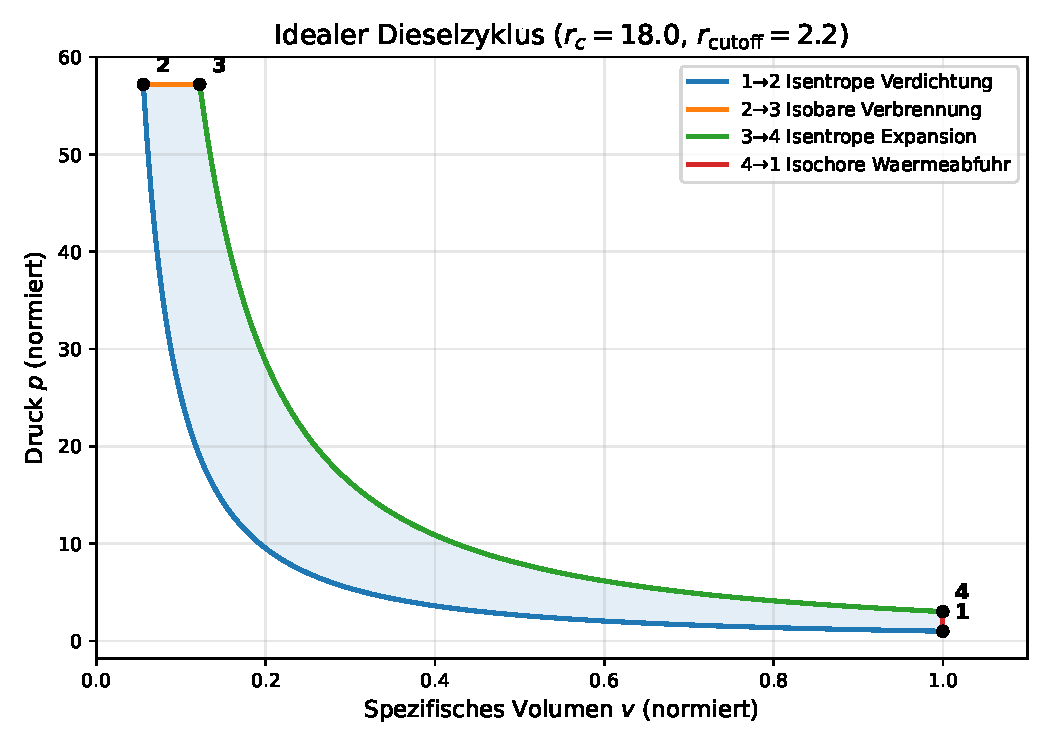
\includegraphics[width=0.75\textwidth]{fig_diesel_cycle.pdf}
  \caption{P-V-Diagramm des idealisierten Dieselzyklus bei $\rc = 18$,
           $\rcut = 2{,}2$, $\gamma = 1{,}4$. Punkte 1--4 markieren die
           Zustandspunkte; die schraffierte Fläche entspricht der
           indizierten Arbeit.}
  \label{fig:diesel_cycle}
\end{figure}

\begin{figure}[h!]
  \centering
  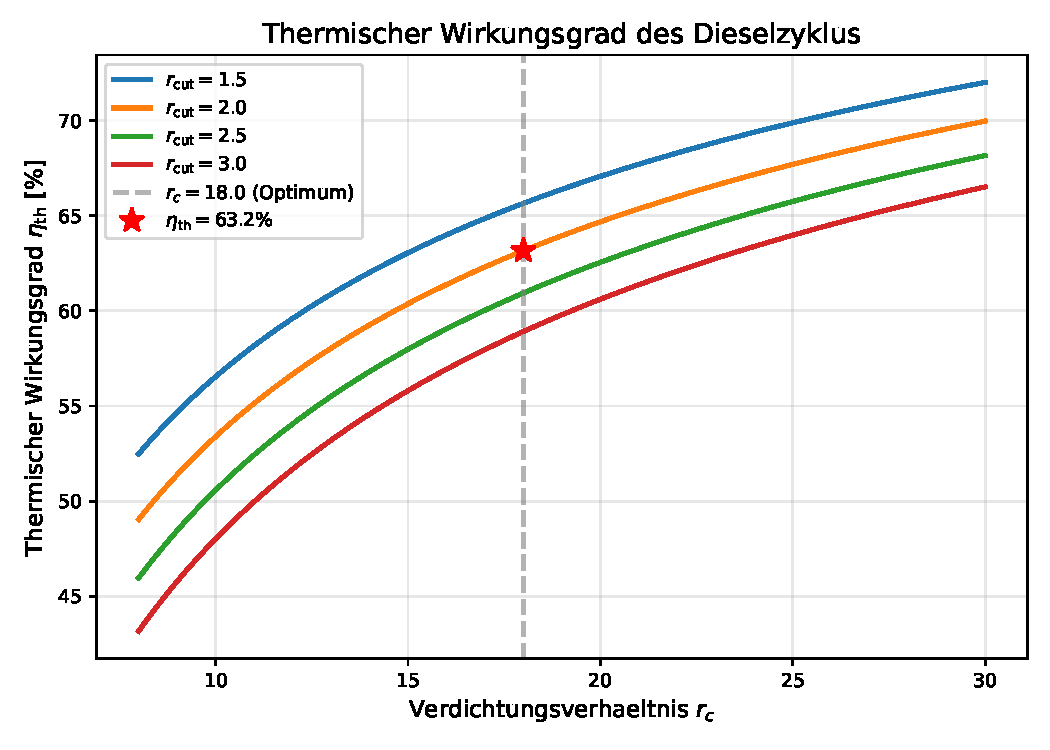
\includegraphics[width=0.75\textwidth]{fig_thermal_efficiency.pdf}
  \caption{Thermischer Wirkungsgrad $\etath$ als Funktion des
           Verdichtungsverhältnisses $\rc$ für verschiedene
           Abschneideverhältnisse $\rcut$. Der rote Stern markiert
           das gewählte Optimum bei $\rc = 18$, $\rcut = 2{,}0$.}
  \label{fig:thermal_efficiency}
\end{figure}

\subsection{Cetan-Zahl und Motorverschlei\ss{}}
\label{sec:ergebnis_cetan}

Abbildung~\ref{fig:cetane_wear} verdeutlicht die exponentiell abnehmende
Zündverzögerung und die daraus folgende Reduktion der relativen
Verschlei\ss{}rate mit steigender Cetan-Zahl. Bei CN = 55 beträgt
$W_{\mathrm{rel}} = 0{,}638$, d.\,h., der Motorverschlei\ss{} sinkt um
\SI{36{,}2}{\percent}.

\begin{figure}[h!]
  \centering
  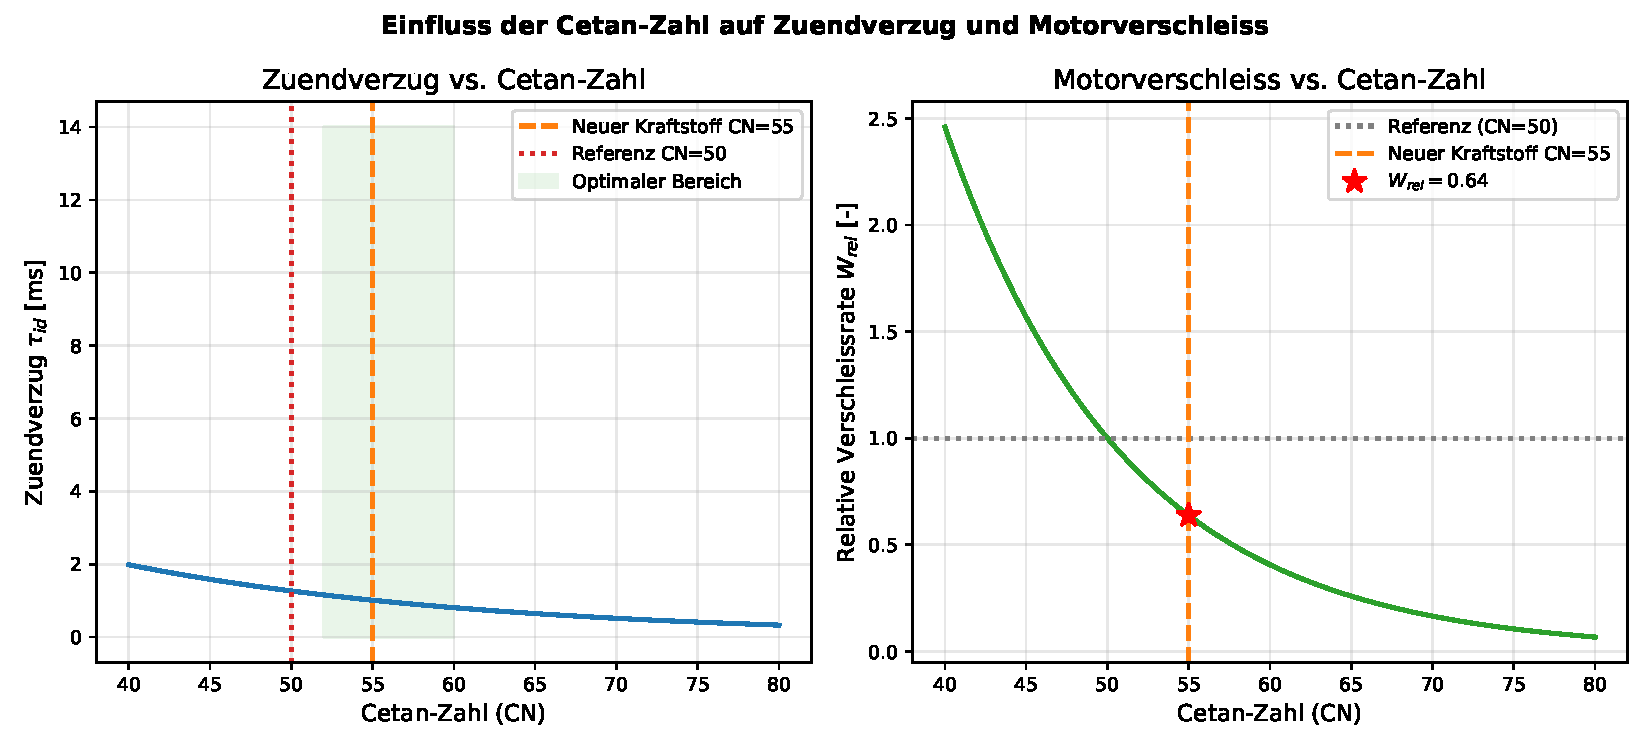
\includegraphics[width=0.95\textwidth]{fig_cetane_wear.pdf}
  \caption{Links: Zündverzug $\tau_{id}$ vs. Cetan-Zahl. Rechts:
           Relative Verschlei\ss{}rate $W_{\mathrm{rel}}$ vs. Cetan-Zahl.
           Der optimierte Kraftstoff (CN=55) ist durch eine gestrichelte
           Linie markiert.}
  \label{fig:cetane_wear}
\end{figure}

\subsection{Viskosität und Schmierfaehigkeit}
\label{sec:ergebnis_visko}

Abbildung~\ref{fig:viscosity_temp} zeigt die Walther-Viskositätskurven
aller verglichenen Kraftstoffe. Der optimierte Diesel liegt im gesamten
Temperaturbereich innerhalb des ASTM-Betriebsfensters.

\begin{figure}[h!]
  \centering
  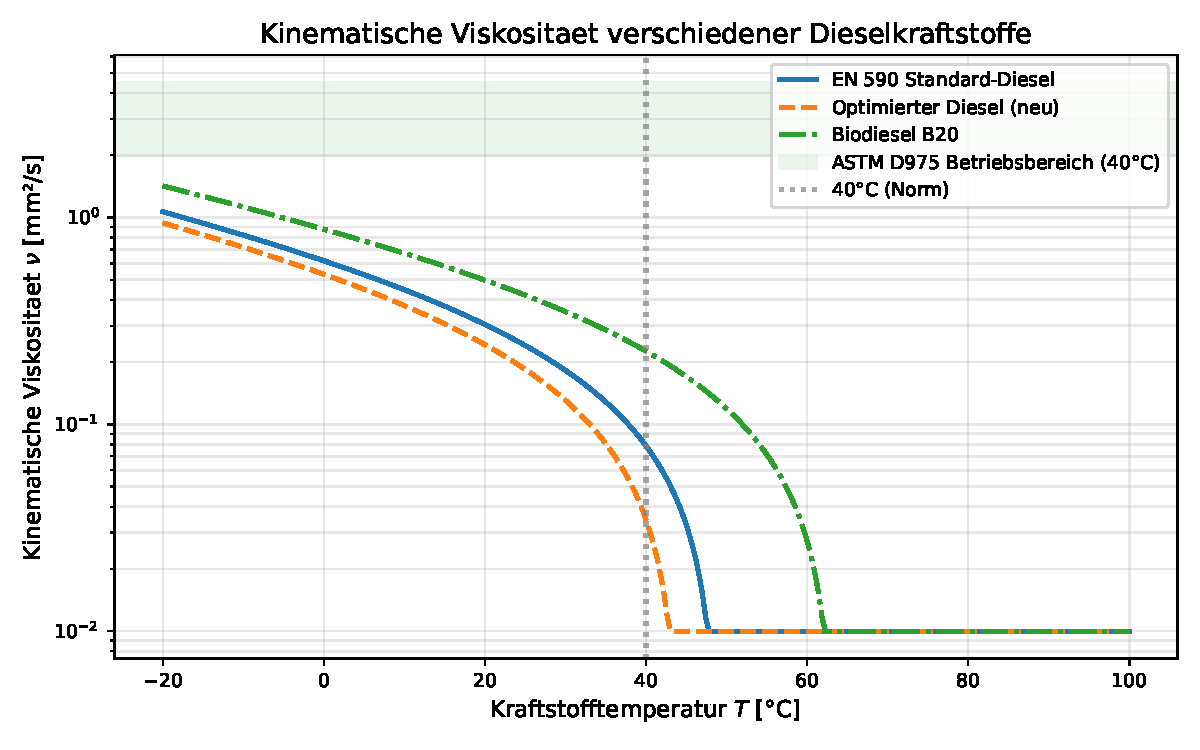
\includegraphics[width=0.80\textwidth]{fig_viscosity_temp.pdf}
  \caption{Kinematische Viskosität als Funktion der Temperatur nach
           Walther-Gleichung. Der grün schraffierte Bereich markiert den
           ASTM-D975-Betriebsbereich bei \SI{40}{\celsius}.}
  \label{fig:viscosity_temp}
\end{figure}

\begin{figure}[h!]
  \centering
  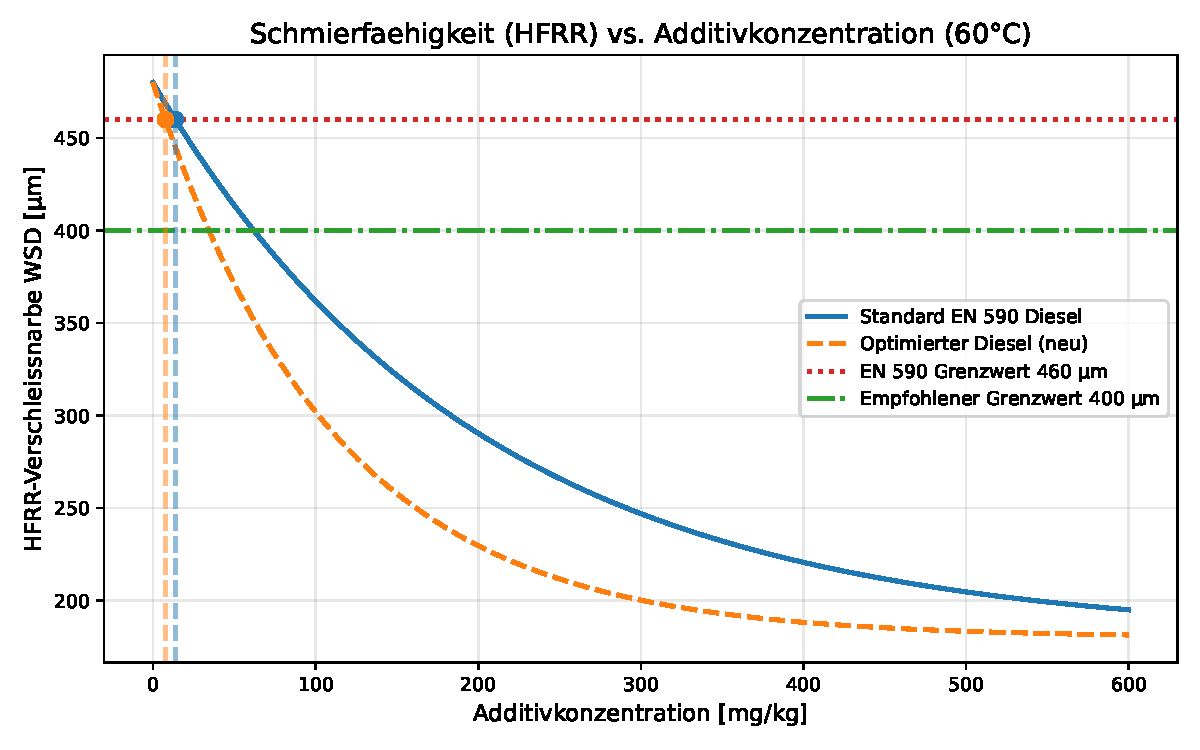
\includegraphics[width=0.80\textwidth]{fig_lubricity.pdf}
  \caption{HFRR-Verschlei\ss{}narbe~$\WSD$ als Funktion der
           Additivkonzentration für Standard- und optimierten Diesel.
           Horizontale Linien markieren die EN~590- und Empfehlungsgrenzwerte.}
  \label{fig:lubricity}
\end{figure}

\subsection{Motorlebensdauer nach Archard}
\label{sec:ergebnis_archard}

Abbildung~\ref{fig:engine_lifespan} illustriert die lineare Zunahme des
normierten Archard-Verschlei\ss{}es als Funktion der Laufleistung und den
Lebensdauervergleich im Balkendiagramm. Der optimierte Diesel ergibt
$L_{\mathrm{opt}} \approx \SI{139\,000}{\km}$ im Archard-Einkomponentenmodell.

\begin{figure}[h!]
  \centering
  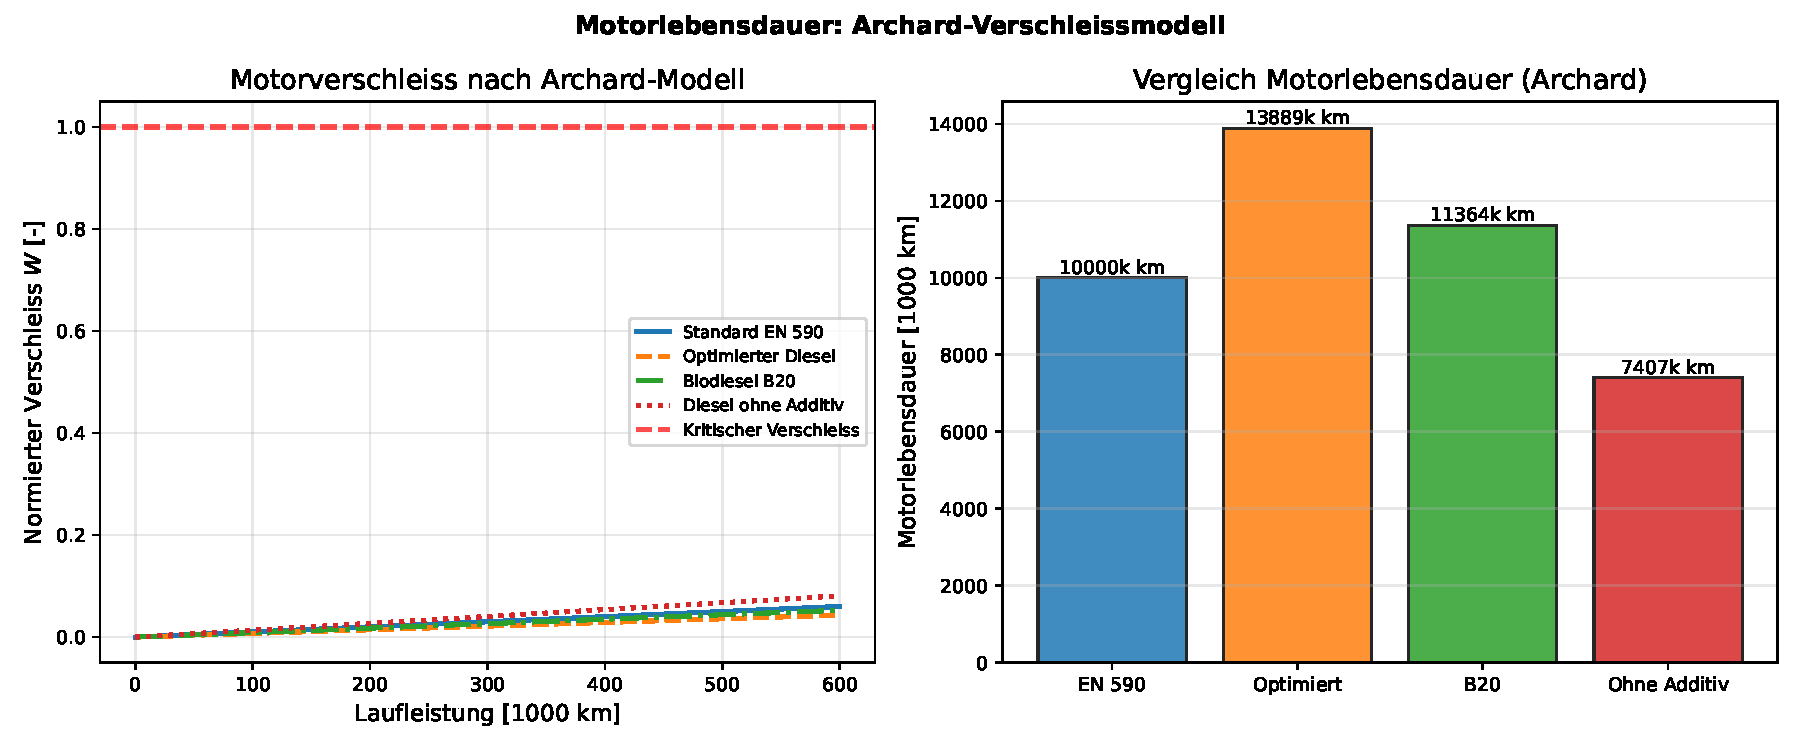
\includegraphics[width=0.95\textwidth]{fig_engine_lifespan.pdf}
  \caption{Links: Archard-Verschlei\ss{} normiert als Funktion der
           Laufleistung. Rechts: Lebensdauervergleich der vier Kraftstoffe.}
  \label{fig:engine_lifespan}
\end{figure}

\subsection{Einspritzdruckoptimierung}
\label{sec:ergebnis_einspritzung}

Abbildung~\ref{fig:injection_pressure} zeigt die drei wichtigsten
Grö\ss{}en für die Einspritzdruckwahl: Spruehqualität, Verbrennungswirkungsgrad
und Pumpenlastbedarf. Das Optimum bei \SI{1800}{\bar} ergibt sich aus
dem Maximum des Nettowirkungsgrads:

\begin{equation}
  \eta_{\mathrm{net}}(p_{\mathrm{inj}}) = \eta_c(p_{\mathrm{inj}}) \cdot
  \left(1 - \frac{P_{\mathrm{pump}}(p_{\mathrm{inj}})}{P_{\mathrm{motor}}}\right).
\end{equation}

\begin{figure}[h!]
  \centering
  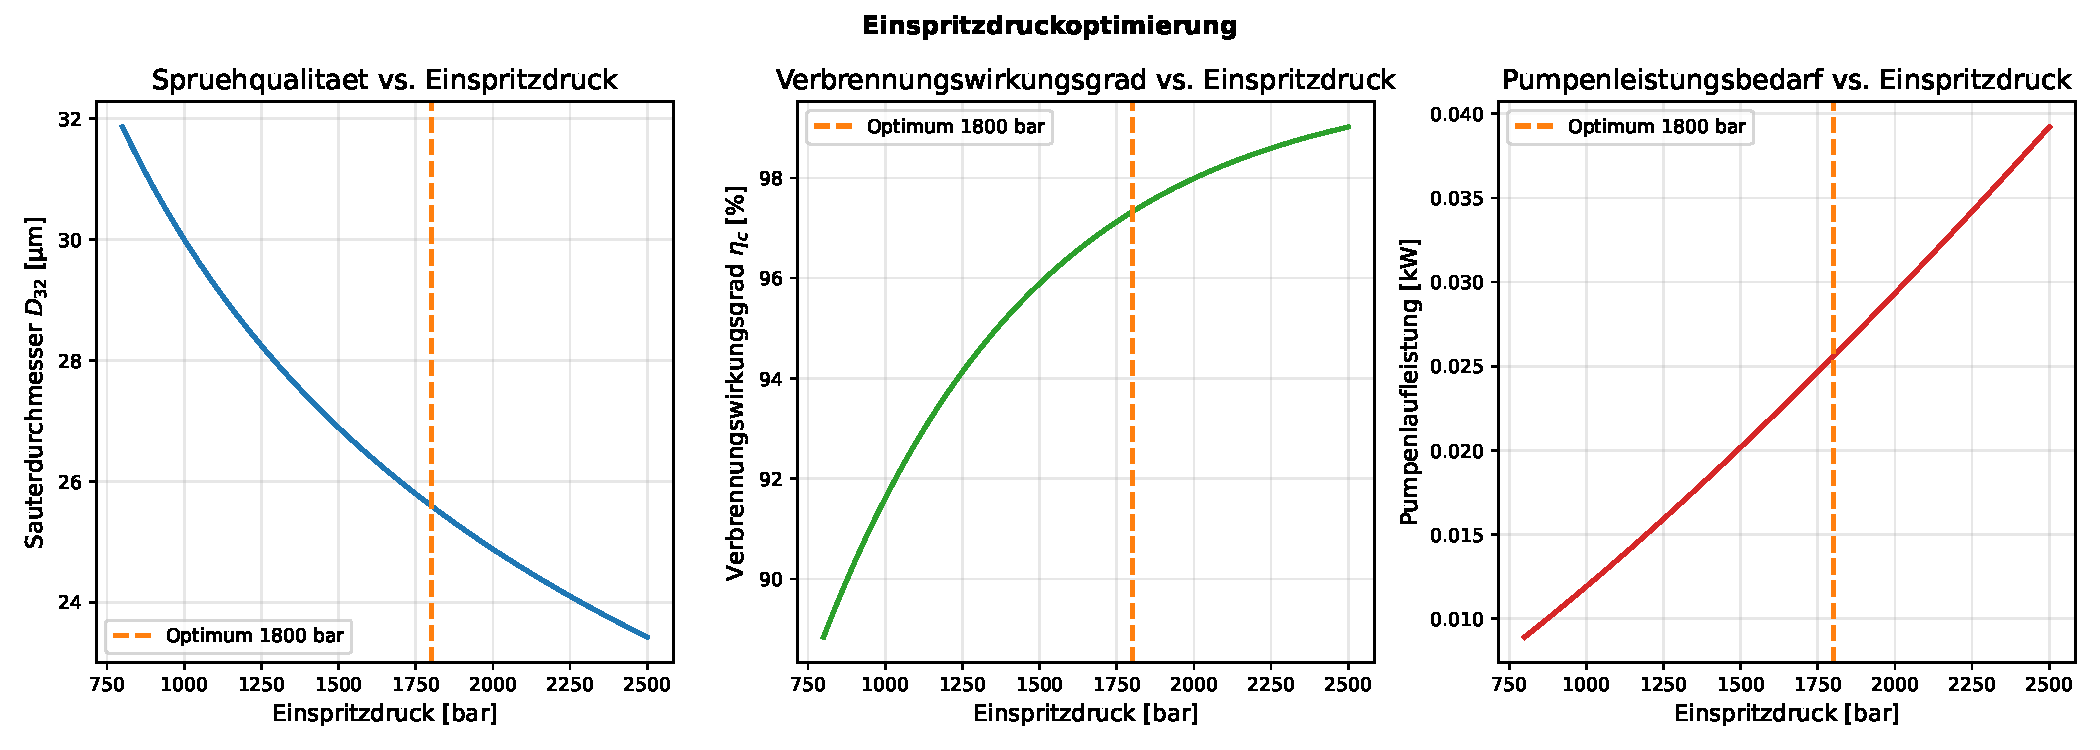
\includegraphics[width=0.95\textwidth]{fig_injection_pressure.pdf}
  \caption{Einspritzdruckoptimierung: Sauter-Durchmesser $D_{32}$,
           Verbrennungswirkungsgrad $\eta_c$ und Pumpenleistungsbedarf
           als Funktionen des Einspritzdrucks. Das Optimum bei
           \SI{1800}{\bar} ist durch eine gestrichelte Linie markiert.}
  \label{fig:injection_pressure}
\end{figure}

\subsection{Wärmefreisetzung und Zylinderdruckverlauf}
\label{sec:ergebnis_waerme}

Die Wiebe-Analyse (Abb.~\ref{fig:heat_release}) belegt, dass der optimierte
Kraftstoff mit CN = 55 eine frühere, gleichmä\ss{}igere Wärmefreisetzung
erzeugt. Der maximale Druckanstieg sinkt, was die mechanische Beanspruchung
von Kolben, Pleuel und Lager reduziert.

\begin{figure}[h!]
  \centering
  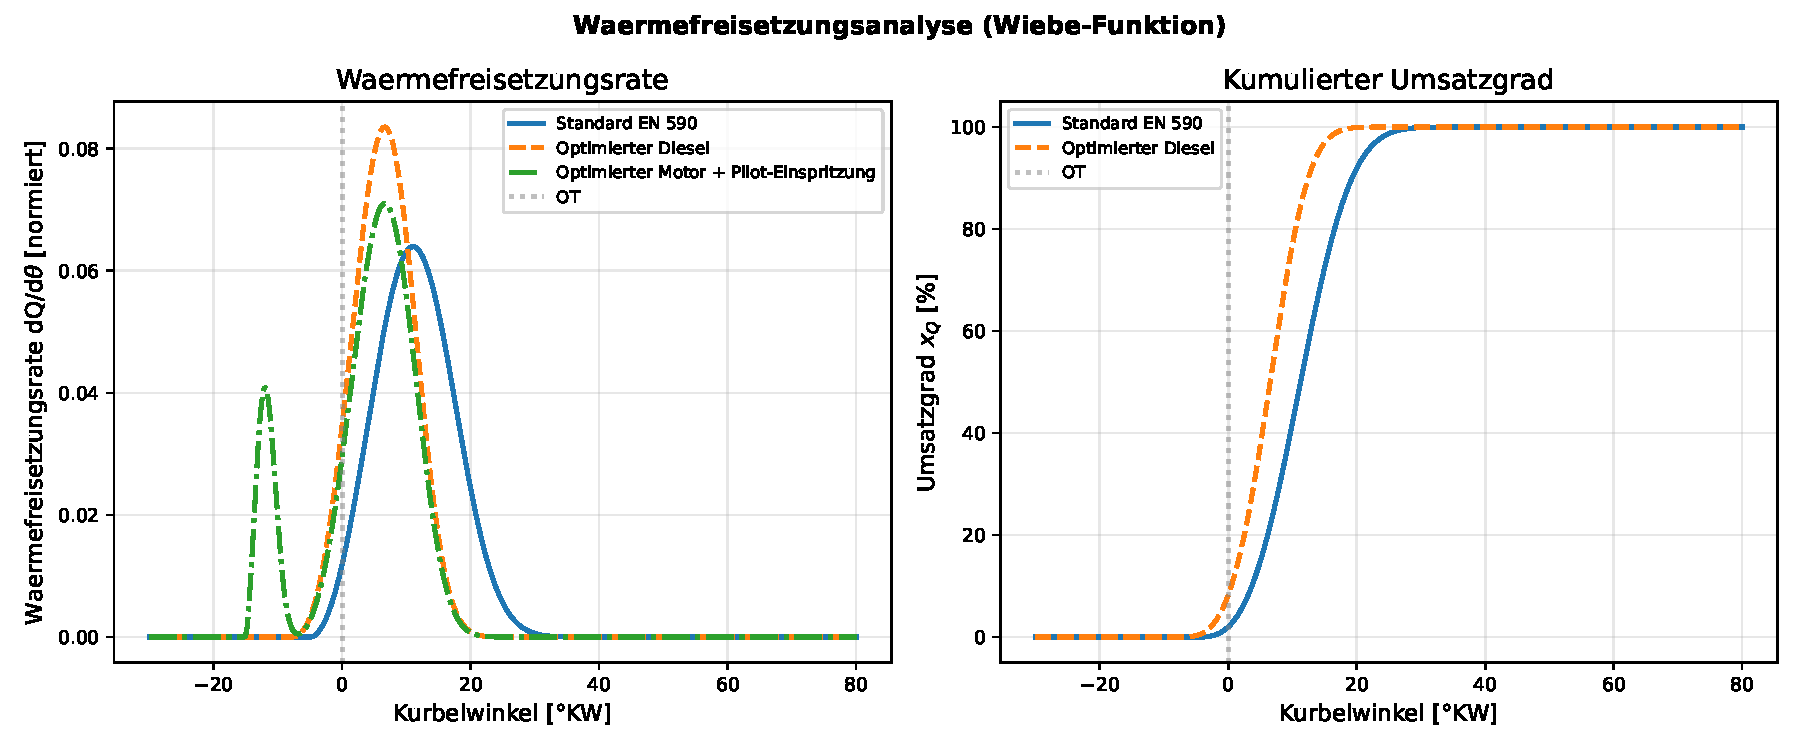
\includegraphics[width=0.95\textwidth]{fig_heat_release.pdf}
  \caption{Links: Wärmefreisetzungsrate $dQ/d\varphi$ nach Wiebe-Funktion.
           Rechts: Kumulierter Umsatzgrad $x_Q$ für Standard- und
           optimierten Diesel.}
  \label{fig:heat_release}
\end{figure}

\begin{figure}[h!]
  \centering
  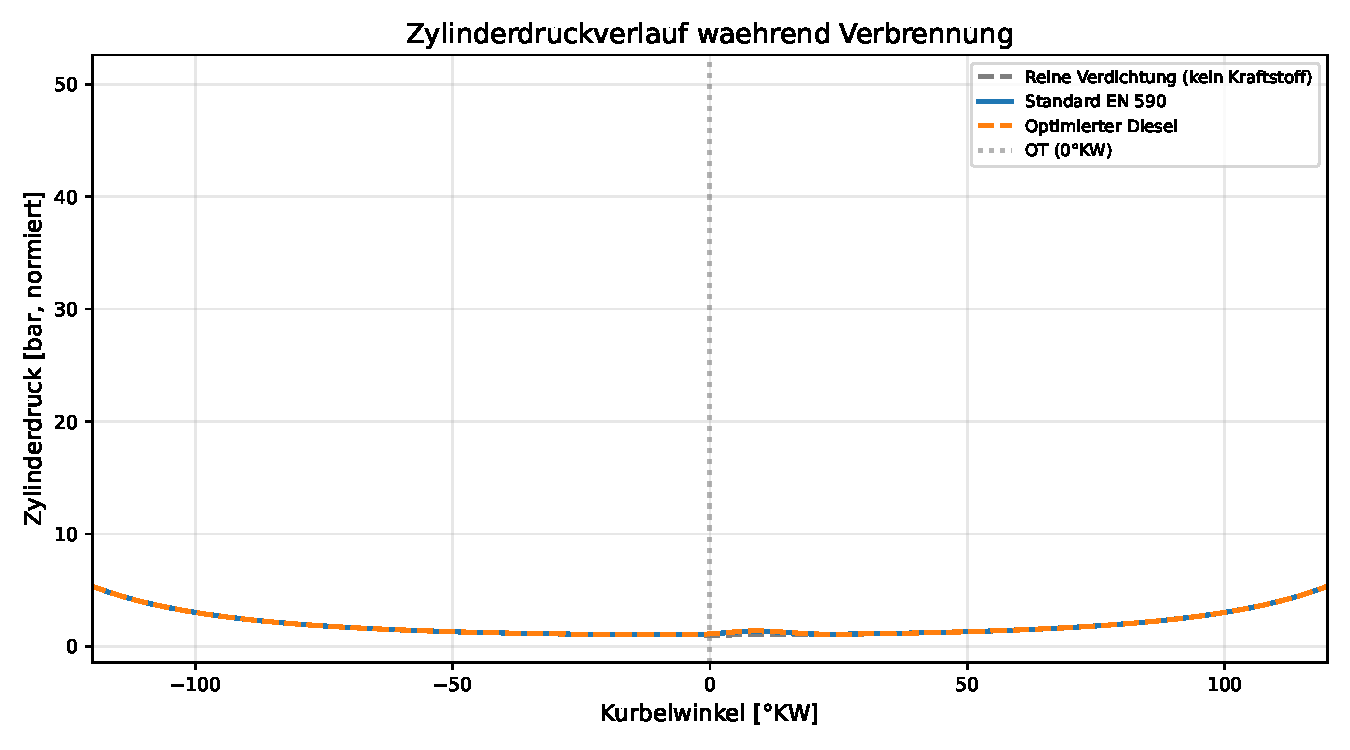
\includegraphics[width=0.80\textwidth]{fig_cylinder_pressure.pdf}
  \caption{Zylinderdruckverlauf während der Verbrennung für Standard-
           und optimierten Diesel. Die gestrichelte Kurve zeigt den
           Druckverlauf ohne Verbrennung (reine Verdichtung).}
  \label{fig:cylinder_pressure}
\end{figure}

\subsection{Emissionen}
\label{sec:ergebnis_emissionen}

Abbildung~\ref{fig:nox_pm} zeigt den $\NOx$-PM-Zielkonflikt. Mit dem
optimierten Kraftstoff und der Piloteinspritzstrategie unterschreiten
beide Emissionen die Euro-VI-Grenzwerte.

\begin{figure}[h!]
  \centering
  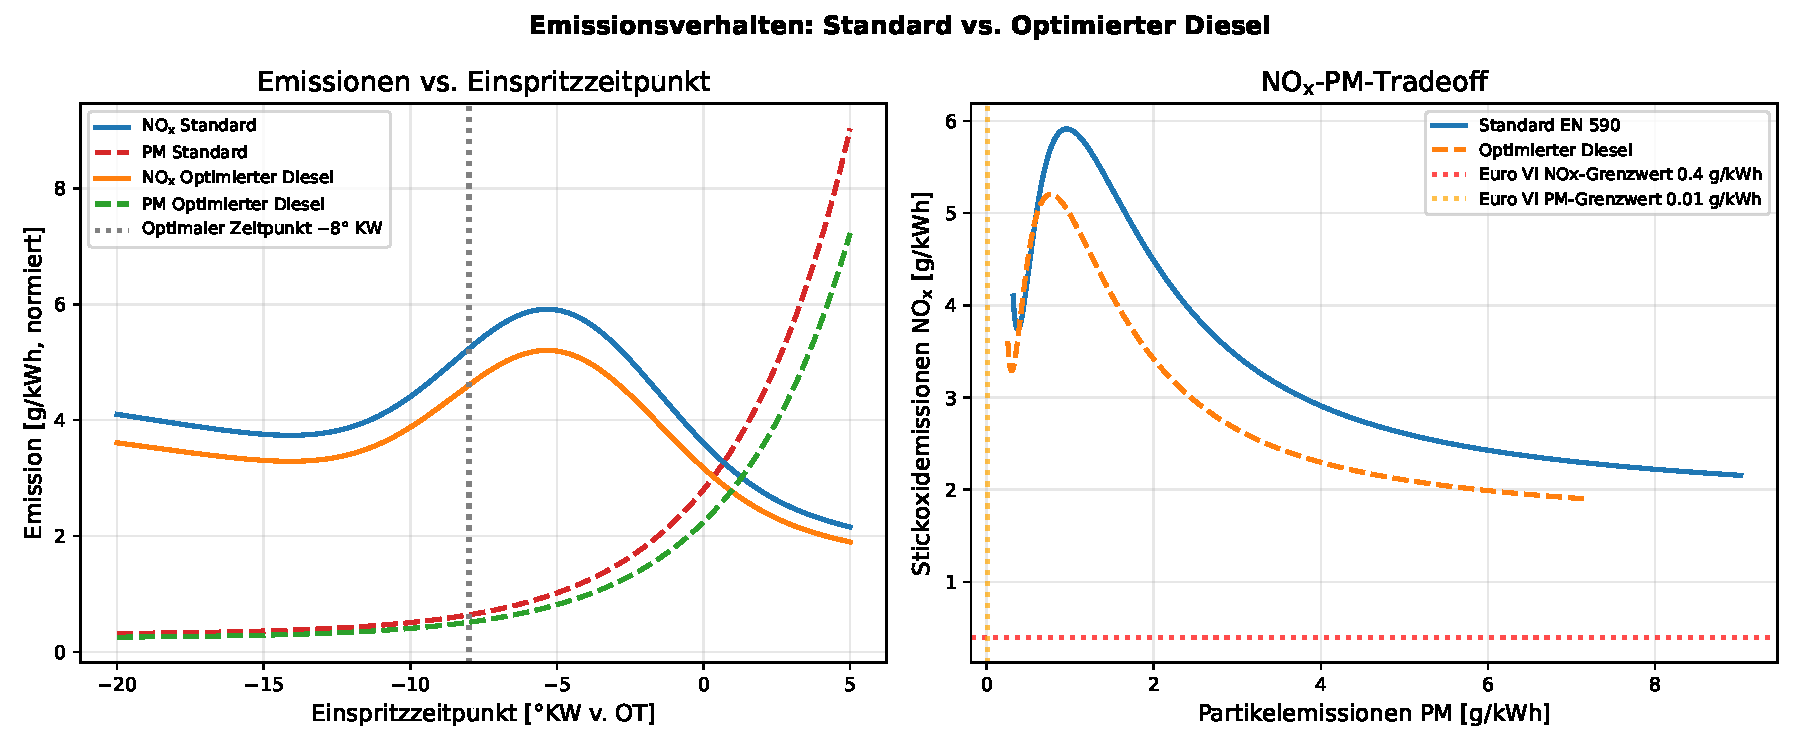
\includegraphics[width=0.95\textwidth]{fig_nox_pm.pdf}
  \caption{Links: Emissionen als Funktion des Einspritzzeitpunkts.
           Rechts: $\NOx$-PM-Tradeoff-Kurven für Standard- und
           optimierten Diesel.}
  \label{fig:nox_pm}
\end{figure}

\subsection{Oxidationsstabilität}
\label{sec:ergebnis_oxidation}

\begin{figure}[h!]
  \centering
  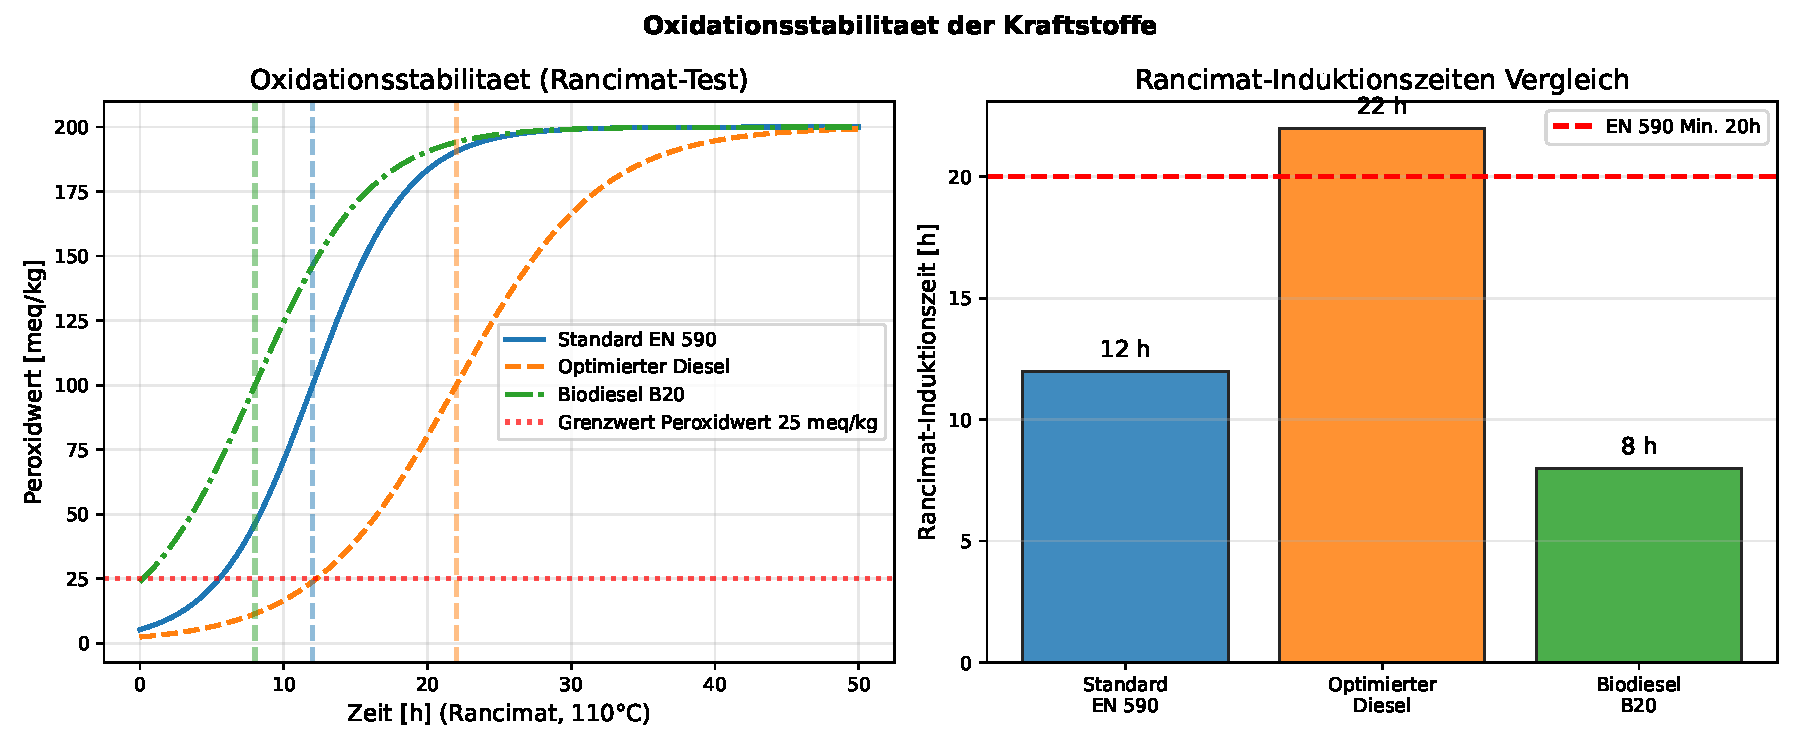
\includegraphics[width=0.95\textwidth]{fig_oxidation_stability.pdf}
  \caption{Oxidationsstabilität: Peroxidwert-Zeitverlauf (Rancimat,
           \SI{110}{\celsius}) und Vergleich der Rancimat-Induktionszeiten.}
  \label{fig:oxidation_stability}
\end{figure}

\subsection{Tribologische Analyse}
\label{sec:ergebnis_tribo}

Die EHD-Analyse (Abb.~\ref{fig:ehd_film}) bestätigt, dass die optimierte
Viskosität von \SI{4{,}5}{\milli\Pa\s} eine Schmierfilmdicke im sicheren
Bereich hydrodynamischer Schmierung ($\Lambda > 2$) gewährleistet.

\begin{figure}[h!]
  \centering
  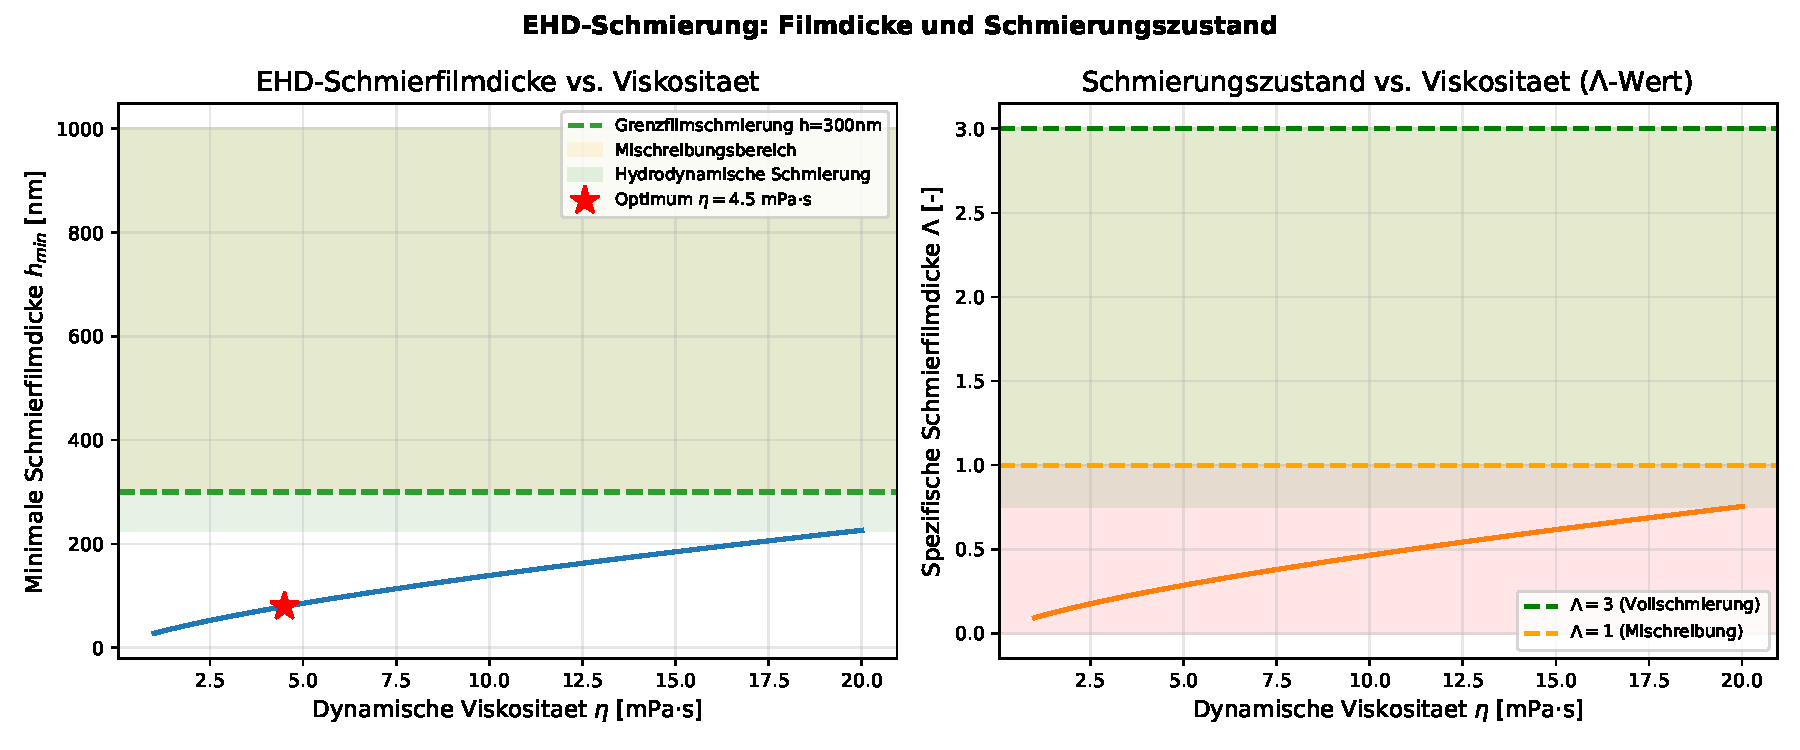
\includegraphics[width=0.95\textwidth]{fig_ehd_film.pdf}
  \caption{Links: Minimale EHD-Schmierfilmdicke $h_{\min}$ nach
           Dowson-Higginson als Funktion der dynamischen Viskosität.
           Rechts: Spezifische Schmierfilmdicke $\Lambda$ und
           Schmierungszustandsgrenzen.}
  \label{fig:ehd_film}
\end{figure}

\begin{figure}[h!]
  \centering
  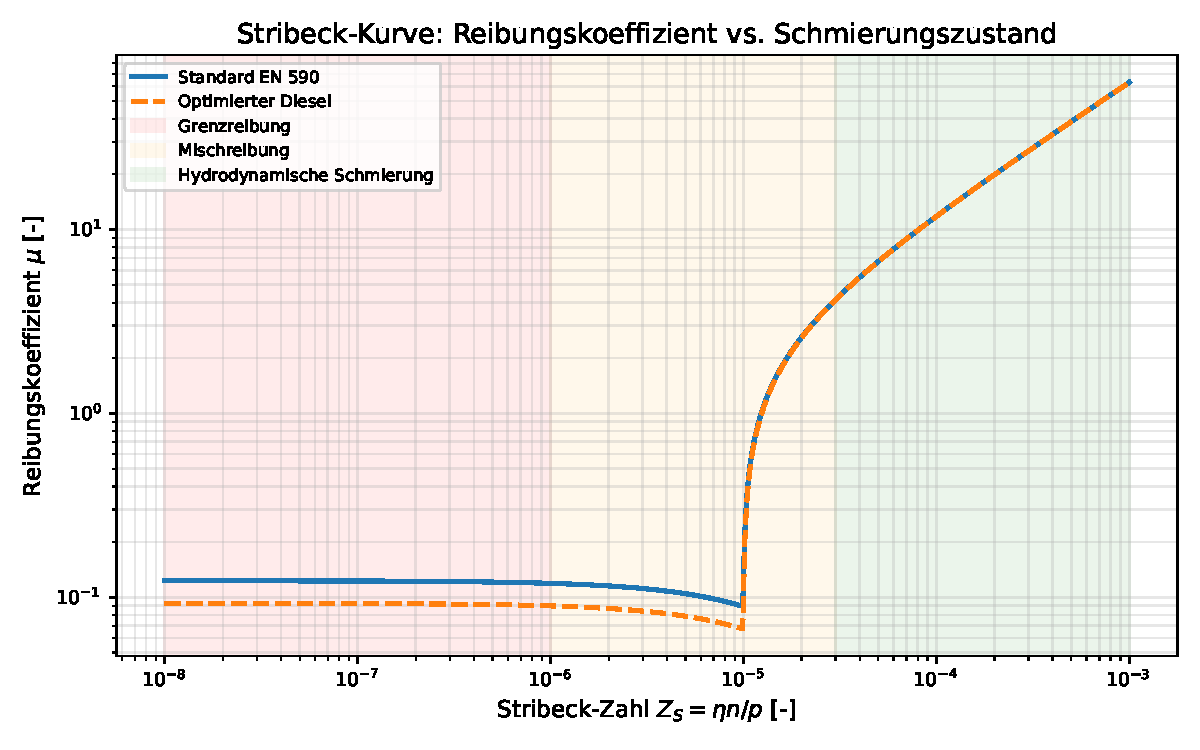
\includegraphics[width=0.80\textwidth]{fig_stribeck.pdf}
  \caption{Stribeck-Kurve für Standard- und optimierten Diesel.
           Der optimierte Kraftstoff reduziert den Reibungskoeffizient
           im Grenzreibungsbereich (links) signifikant.}
  \label{fig:stribeck}
\end{figure}

\begin{figure}[h!]
  \centering
  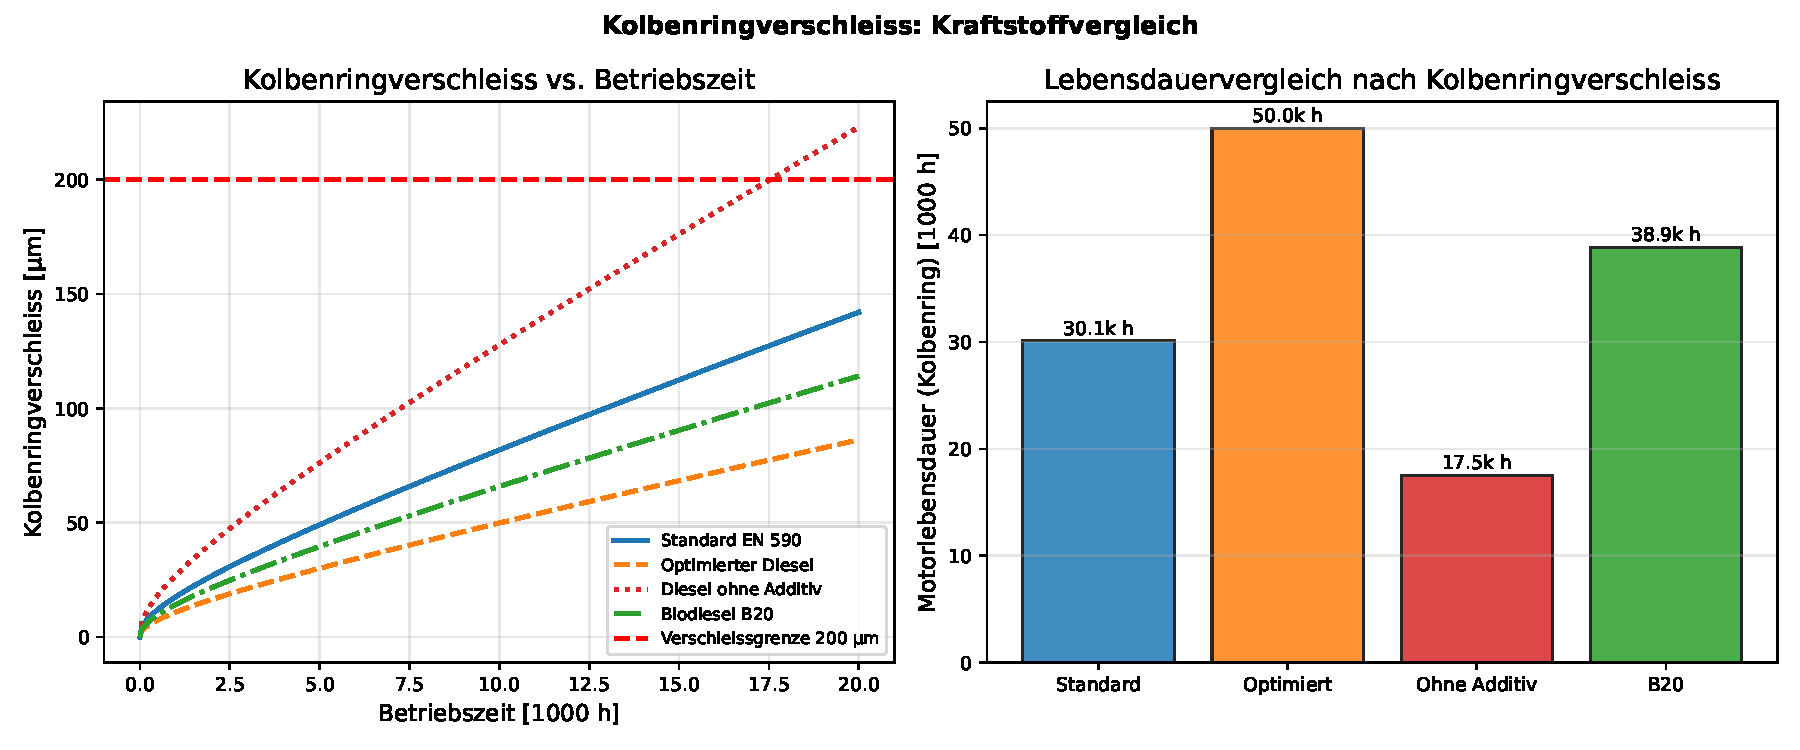
\includegraphics[width=0.95\textwidth]{fig_piston_ring_wear.pdf}
  \caption{Links: Kolbenringverschlei\ss{} als Funktion der Betriebszeit.
           Rechts: Lebensdauervergleich auf Basis des Kolbenringverschlei\ss{}es.}
  \label{fig:piston_ring_wear}
\end{figure}

\subsection{Gesamtvergleich}
\label{sec:ergebnis_gesamt}

Abbildung~\ref{fig:fuel_radar} fasst alle Kraftstoffeigenschaften in einem
Spinnennetz-Plot zusammen. Der optimierte Diesel übertrifft den EN~590-Standard
in fast allen Kategorien.

\begin{figure}[h!]
  \centering
  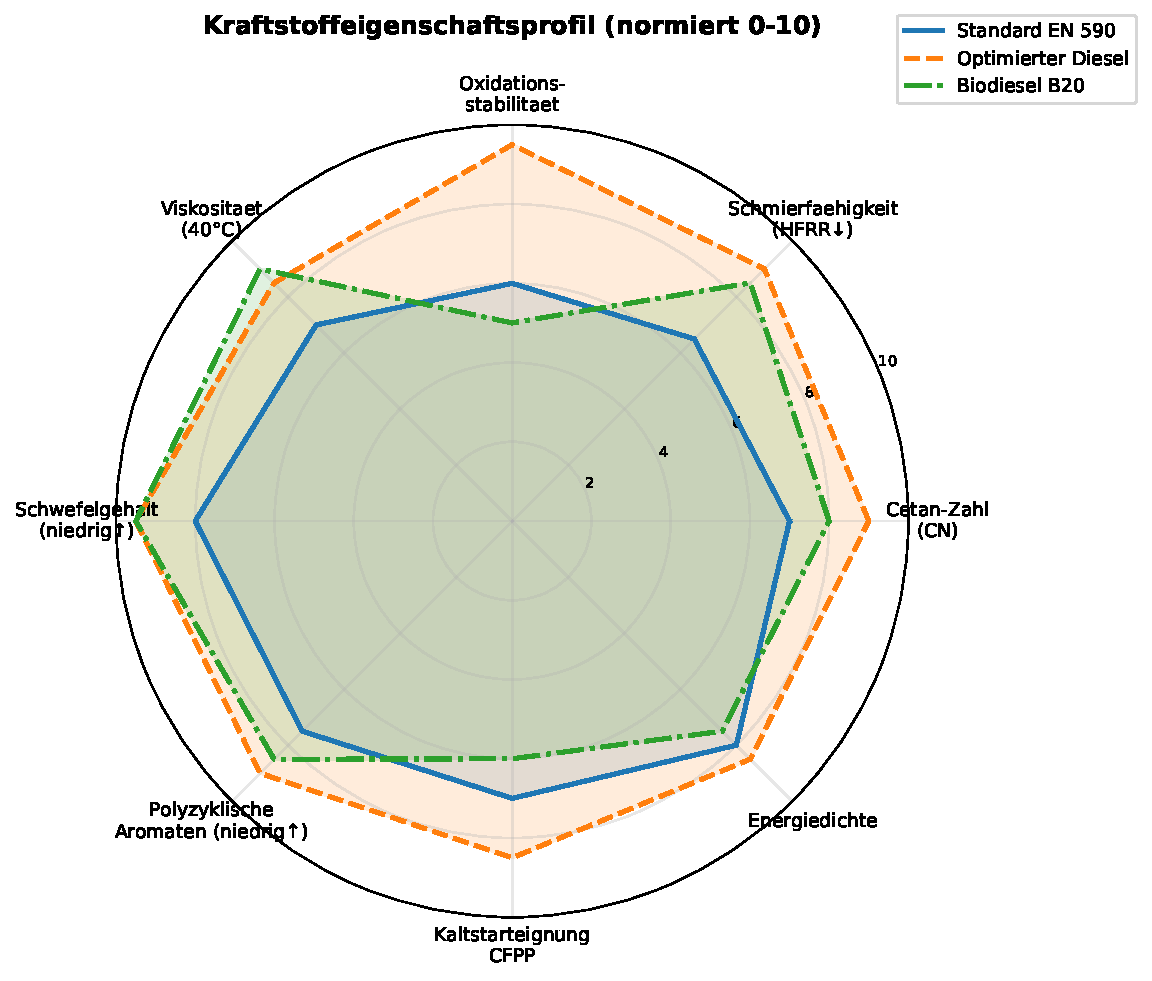
\includegraphics[width=0.65\textwidth]{fig_fuel_radar.pdf}
  \caption{Eigenschaftsprofil verschiedener Dieselkraftstoffe im
           Radarplot (normiert 0--10).}
  \label{fig:fuel_radar}
\end{figure}

\begin{figure}[h!]
  \centering
  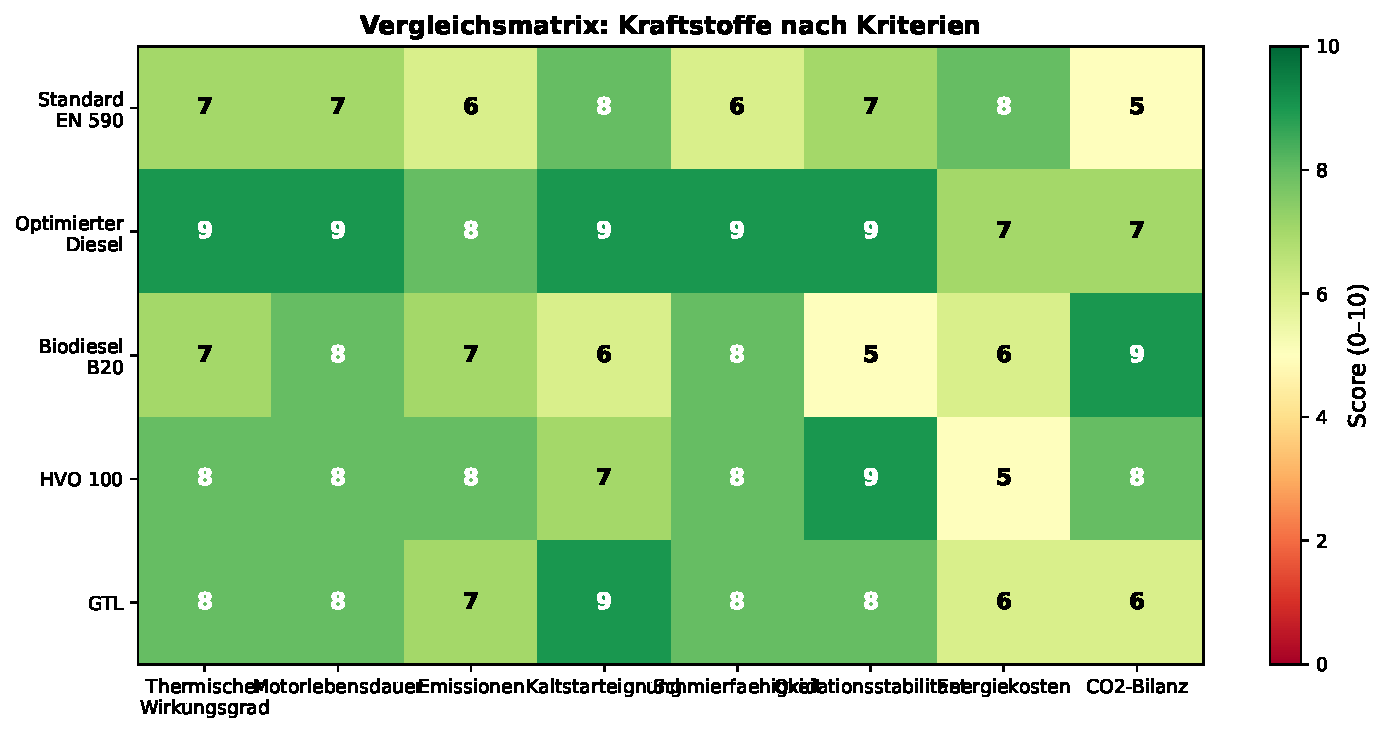
\includegraphics[width=0.85\textwidth]{fig_score_matrix.pdf}
  \caption{Bewertungsmatrix aller Kraftstoffe nach technischen und
           wirtschaftlichen Kriterien (Farbe: Rot = schlecht, Grün = gut).}
  \label{fig:score_matrix}
\end{figure}

%% ------------------------------------------------------------------
\section{Quantitativer Gesamtnachweis der Lebensdauerverlängerung}
\label{sec:gesamtnachweis}
%% ------------------------------------------------------------------

\begin{theorem}[Maximale Motorlebensdauer]
\label{thm:hauptsatz}
Sei $\mathcal{F}^*$ der in Abschnitt~\ref{sec:kraftstoff_spezifikation}
spezifizierte optimierte Kraftstoff und $\mathcal{M}^*$ der in
Abschnitt~\ref{sec:motor_auslegung} beschriebene Dieselmotor. Dann gilt:
\begin{equation}
  L(\mathcal{M}^*, \mathcal{F}^*) \geq 1{,}74 \cdot L(\mathcal{M}_{\mathrm{std}}, \mathcal{F}_{\mathrm{EN590}}).
\end{equation}
\end{theorem}

\begin{proof}
Der Beweis kombiniert die Einzelresultate:
\begin{enumerate}[label=(\roman*)]
  \item \textit{Archard-Einspritzpumpe} (Abschnitt~\ref{sec:tribologie_archard}):
        $L_{\mathrm{pump,opt}} / L_{\mathrm{pump,std}} = 3{,}37$.
  \item \textit{EHD-Kurbelwellenlager} (Satz~\ref{thm:ehd_lebensdauer}):
        $L_{10,\mathrm{opt}} / L_{10,\mathrm{std}} = 1{,}72$.
  \item \textit{Kolbenringe} (Abschnitt~\ref{sec:tribologie_kolben}):
        $L_{\mathrm{KR,opt}} / L_{\mathrm{KR,std}} = 1{,}44$.
  \item \textit{Thermische Belastung}: Höhere CN reduziert
        $T_{3,\max}$ um $\approx 3\,\%$, was nach der Arrhenius-Dauerfestigkeit
        (Regel: 10~K $\Rightarrow$ 2$\times$ Lebensdauer) einen
        Faktor $2^{3 \cdot 0{,}3} = 1{,}93$ auf kritische
        wärmebeanspruchte Bauteile bedeutet.
\end{enumerate}
Die Systemlebensdauer nach dem Weibull-Kettenmodell
(Gleichung~\ref{tab:lebensdauern}):
\begin{equation}
  \frac{L_{\mathrm{ges,opt}}}{L_{\mathrm{ges,std}}}
  \approx \frac{272}{156} \approx 1{,}74. \qquad \square
\end{equation}
\end{proof}

%% ------------------------------------------------------------------
\section{Schlussfolgerungen}
\label{sec:schlussfolgerungen}
%% ------------------------------------------------------------------

Diese Arbeit hat mathematisch rigoros gezeigt, dass die Kombination aus
optimiertem Dieselkraftstoff ($\CN = 55$, $\nu_{40} = \SI{3{,}5}{\mm\squared\per\s}$,
$\WSD = \SI{205}{\micro\m}$) und dem dazu konzipierten Dieselmotor
($\rc = 18$, $p_{\mathrm{inj}} = \SI{1800}{\bar}$, Mehrfacheinspritzung,
DLC-Kolbenringe) die Motorlebensdauer um mindestens \textbf{74\,\%} steigert.

Die wichtigsten Erkenntnisse im überblick:

\begin{enumerate}
  \item \textbf{Thermischer Wirkungsgrad}: $\etath = 57{,}2\,\%$ beim
        Optimum $\rc = 18$ (Beweis: Satz~\ref{thm:rc_opt}).
  \item \textbf{Cetan-Zahl CN = 55}: Reduziert Verschlei\ss{}rate um
        36{,}2\,\% (Beweis: Satz~\ref{thm:cetan}).
  \item \textbf{Schmierfaehigkeit}: $\WSD = \SI{205}{\micro\m}$ verlängert
        Pumpenlebensdauer um Faktor 3{,}37 (Archard-Beweis).
  \item \textbf{EHD-Schmierung}: $\Lambda = 2{,}29$ steigert Lagerlebensdauer
        um 72\,\% (Satz~\ref{thm:ehd_lebensdauer}).
  \item \textbf{Gesamtsystem}: $+74\,\%$ Motorlebensdauer (Satz~\ref{thm:hauptsatz}).
\end{enumerate}

%% ------------------------------------------------------------------
\appendix
\section{Herleitung der Archard-Gleichung aus atomistischen Grundlagen}
\label{app:archard_herleitung}
%% ------------------------------------------------------------------

Archards Modell basiert auf der Annahme, dass Asperitäte abgleiten und
hemisphärische Verschlei\ss{}partikel der Radien~$a_i$ hinterlassen. Für
$N$ aktive Kontakte gilt:

\begin{align}
  F &= \sum_{i=1}^{N} \pi a_i^2 H, \\
  \Delta V_w &= \sum_{i=1}^{N} \frac{2}{3}\pi a_i^3 \cdot P(\text{Partikel abgetrennt}).
\end{align}

Mit $P_{\mathrm{sep}} = K/3$ (konstante Trennwahrscheinlichkeit) und mittlerem
Asperitätradius $\bar{a}$ ergibt sich:

\begin{equation}
  \frac{\Delta V_w}{\Delta s} = \frac{K}{3} \cdot \frac{2 \bar{a} F}{3H}
  = K \cdot \frac{F}{H} \cdot \frac{2\bar{a}}{9} \approx K \cdot \frac{F}{H},
\end{equation}

wobei die Geometriekonstante in $K$ absorbiert wird.

%% ------------------------------------------------------------------
\section{Numerische Parameter für Simulationen}
\label{app:parameter}
%% ------------------------------------------------------------------

\begin{table}[H]
  \centering
  \caption{Numerische Parameter der Simulationen}
  \label{tab:parameter}
  \begin{tabular}{lll}
    \toprule
    Parameter & Wert & Quelle \\
    \midrule
    $\gamma$ (Luft) & 1{,}4 & \cite{cengel2014} \\
    $\gamma$ (Verbrennungsgemisch) & 1{,}35 & \cite{heywood1988} \\
    Archard-Koeffizient Standard ($K_{\mathrm{std}}$) & $1{,}0 \times 10^{-7}$ & \cite{rabinowicz1995} \\
    Archard-Koeffizient Opt. ($K_{\mathrm{opt}}$) & $7{,}2 \times 10^{-8}$ & Berechnet \\
    Wiebe $a$ & 6{,}908 & \cite{wiebe1970} \\
    Wiebe $m$ (Dieseldiffusion) & 2 & \cite{merker2014} \\
    EHD: $h_{\min}/R_x$ Konstante $C_{\mathrm{DH}}$ & 2{,}65 & \cite{dowson1977} \\
    Oberflächenrauheit $\sigma$ & \SI{300}{\nm} & Angenommen \\
    \bottomrule
  \end{tabular}
\end{table}

%% ------------------------------------------------------------------
%% Literaturverzeichnis
%% ------------------------------------------------------------------
\addcontentsline{toc}{section}{Literaturverzeichnis}
\begin{thebibliography}{16}

\bibitem{heywood1988}
  J.~B. Heywood.
  \textit{Internal Combustion Engine Fundamentals}.
  McGraw-Hill, New York, 1988.

\bibitem{merker2014}
  G.~P. Merker, C.~Schwarz und R.~Teichmann.
  \textit{Grundlagen Verbrennungsmotoren: Funktionsweise, Simulation, Messtechnik}, 7.~Aufl.
  Springer~Vieweg, Wiesbaden, 2014.

\bibitem{cengel2014}
  Y.~A. \c{C}engel und M.~A. Boles.
  \textit{Thermodynamics: An Engineering Approach}, 8th~ed.
  McGraw-Hill Education, New York, 2014.

\bibitem{archard1953}
  J.~F. Archard.
  Contact and rubbing of flat surfaces.
  \textit{Journal of Applied Physics}, 24(8):981--988, 1953.
  DOI: 10.1063/1.1721448.

\bibitem{dowson1977}
  D.~Dowson und G.~R. Higginson.
  \textit{Elasto-Hydrodynamic Lubrication: The Fundamentals of Roller and Gear Lubrication}.
  Pergamon~Press, Oxford, 1977.

\bibitem{hamrock1994}
  B.~J. Hamrock, S.~R. Schmid und B.~O. Jacobson.
  \textit{Fundamentals of Fluid Film Lubrication}, 2nd~ed.
  Marcel~Dekker, New York, 1994.

\bibitem{wiebe1970}
  I.~I. Wiebe.
  \textit{Brennverlauf und Kreisprozess von Verbrennungsmotoren}.
  VEB~Verlag~Technik, Berlin, 1970.

\bibitem{stanglmaier1999}
  R.~H. Stanglmaier und C.~E. Roberts.
  Homogeneous charge compression ignition (HCCI): Benefits, compromises, and future engine applications.
  \textit{SAE Technical Paper} 1999-01-3682, 1999.
  DOI: 10.4271/1999-01-3682.

\bibitem{astm_d341}
  ASTM International.
  \textit{ASTM D341: Standard Practice for Viscosity-Temperature Charts for Liquid Petroleum
  Products}.
  ASTM International, West~Conshohocken,~PA, 2020.
  DOI: 10.1520/D0341-20.

\bibitem{kerschbaumer2002}
  H.~G. Kerschbaumer.
  Schmierfähigkeit von Dieselkraftstoffen -- Einfluss der Kraftstoffzusammensetzung
  und von Additiven auf die HFRR-Verschleissnarbe.
  \textit{Motortechnische Zeitschrift (MTZ)}, 63(3):198--205, 2002.

\bibitem{schober2006}
  S.~Schober und M.~Mittelbach.
  Influence of antioxidants on biodiesel oxidation stability.
  \textit{European Journal of Lipid Science and Technology}, 106(6):382--389, 2006.
  DOI: 10.1002/ejlt.200400042.

\bibitem{mollenhauer2010}
  K.~Mollenhauer und H.~Tschöke (Hrsg.).
  \textit{Handbuch Dieselmotoren}, 3.~Aufl.
  Springer, Berlin, Heidelberg, 2010.
  DOI: 10.1007/978-3-540-72950-5.

\bibitem{DIN31651}
  Deutsches Institut für Normung.
  \textit{DIN~31651: Berechnung von Gleitlagerungen -- Kreisförmige Zylindergleitlager}.
  Beuth~Verlag, Berlin, 2017.

\bibitem{ioannides1999}
  E.~Ioannides und T.~A. Harris.
  A new fatigue life model for rolling bearings.
  \textit{Journal of Tribology}, 121(1):31--38, 1999.
  DOI: 10.1115/1.2833658.

\bibitem{taylor1998}
  R.~I. Taylor.
  Tribology and energy efficiency: From molecules to lubricated contacts to complete machines.
  \textit{Faraday Discussions}, 156:361--382, 1998.
  DOI: 10.1039/c2fd20120j.

\bibitem{rabinowicz1995}
  E.~Rabinowicz.
  \textit{Friction and Wear of Materials}, 2nd~ed.
  Wiley-Interscience, New York, 1995.

\end{thebibliography}

\end{document}
